% !TEX root = SystemTemplate.tex

\chapter{Design  and Implementation}
This section is used to describe the design details for each of the major components in the system. The autonomous systems of teh UAV can be broken into individual components and the following sections will be divided by such. The first section will cover our simulation environment, the second will cover the autonomous takeoff and waypoint navigation, the third section will discuss our two autonomous landing approaches, and finally the fourth section will cover the UAV.      

\section{Simulation Environment}
\subsection{Technologies  Used}
The simulation environment will be implemented using Gazebo as the actual environment itself and will use ROS so we can use the message passing services to communicate with different modules of code that will be written. This environment will handle all testing so nothing is tested on the physical UAV until it is verified working in a simulated environment that utilizes a pixhawk.
\subsection{Component  Overview}
\begin{itemize}
  \item Ubuntu 14.04 LTS
  \item Gazebo
  \item Mavlink
  \item python
  \item c++
  \item R.O.S.
  \item Mavros (Ros wrapper around Mavlink)
\end{itemize}
\subsection{Phase Overview}
The simulation environment is still a work in progress on setting up communication with a simulated pixhawk with software in the loop (SITL), however as soon as the pixhawk is received hardware in the loop (HITL) will be attempted because of issues simulating the device. Issues as of now are loading a waypoint file and sending commands. A file checksum appears to be invalid for the waypoint file and a invalid flight controller unit is returned after sending commands to the simulated pixhawk with the mavros cmd node.
\subsection{Design Details}
Currently the Design for the simulation is relying on outside sources for installing the environment and setting up packages. These details are discussed in the Prototype section within sprint report \#3.


\section{Autonomous Takeoff and Waypoint Navigation} 
\subsection{Technologies  Used}
The autonomous takeoff and waypoint navigation system is separate from the simulation environment and landing approaches because these will be contained in a mission that will be uploaded into the pixhawk. There will be a waypoint publisher (wpt\_pub) node that will receive input from a user and create a mission file out of that input. Another module within the node will start publishing waypoints to the node so that it nodes what path to take what to do using mavros messages.
\subsection{Component  Overview}
wpt\_pub dependencies:
\begin{itemize}
  \item Ubuntu 14.04 LTS
  \item python
  \item c++
  \item R.O.S.
  \item Mavros
  \item Mavros msgs
\end{itemize}
\subsection{Phase Overview}
The wpt\_pub node can currently publish mavros messages that contain take off, land, and arm commands successfully, however the simulated pixhawk reports back that it is an invalid flight controller unit most times. It does receive waypoints successfully through mavros messages.
\subsection{Design Details}
\lstinputlisting[language=C++]{code/wpt_pub.hpp}
\lstinputlisting[language=C++]{code/wpt_pub.cpp}
\lstinputlisting[language=C++]{code/wpt_pub_node.cpp}

\newpage
\section{Landing Approaches}
\subsection{Visual Homography}
One of the approaches we will be using for the task of landing the UAV will be using visual homography. The basic goal here is to take an image that will contain the landing pad, and, based on the how the target looks on the pad, determine range to pad, orientation with respect to the pad, and the angle above the horizon with respect to the pad. This information will then be used to determine how to actually fly the UAV so that it will be able to safely land on the pad.
\subsubsection{Technologies  Used}
In order to accomplish this, we will use a number of tools. First and foremost, we will be using OpenCV as our image recognition library. OpenCV is a powerful open-source toolkit that will be able to handle any image processing that we need to do. The algorithm will be developed in Python, as this provides an easy-to-understand syntax, and will be able to deliver the performance that we need.
\subsubsection{Component  Overview}
\begin{itemize}
	\item Ubuntu 14.04 LTS
	\item Python
	\item OpenCV
\end{itemize}
\subsubsection{Phase Overview}
The algorithm is still a work in progress, but steps have been made. We have been able to compile and run last year's code, and have a working blob detection system up and running. This system is able to detect a pad with three colored circles by looking for the colors of the circles. The circles are red, green, and blue. It is then able to calculate the distance to the target, since it knows what size the target should be. This should be very helpful moving forward, as we are able to find the pad. In the coming sprints, we will attempt to move toward a pad that has four circles, as we believe this will give us more information to use for our homography computations.
\subsubsection{Design Details}
In the following image, you can see results from last year's code running and detecting the colored circles on a large target with three circles.

\begin{center} 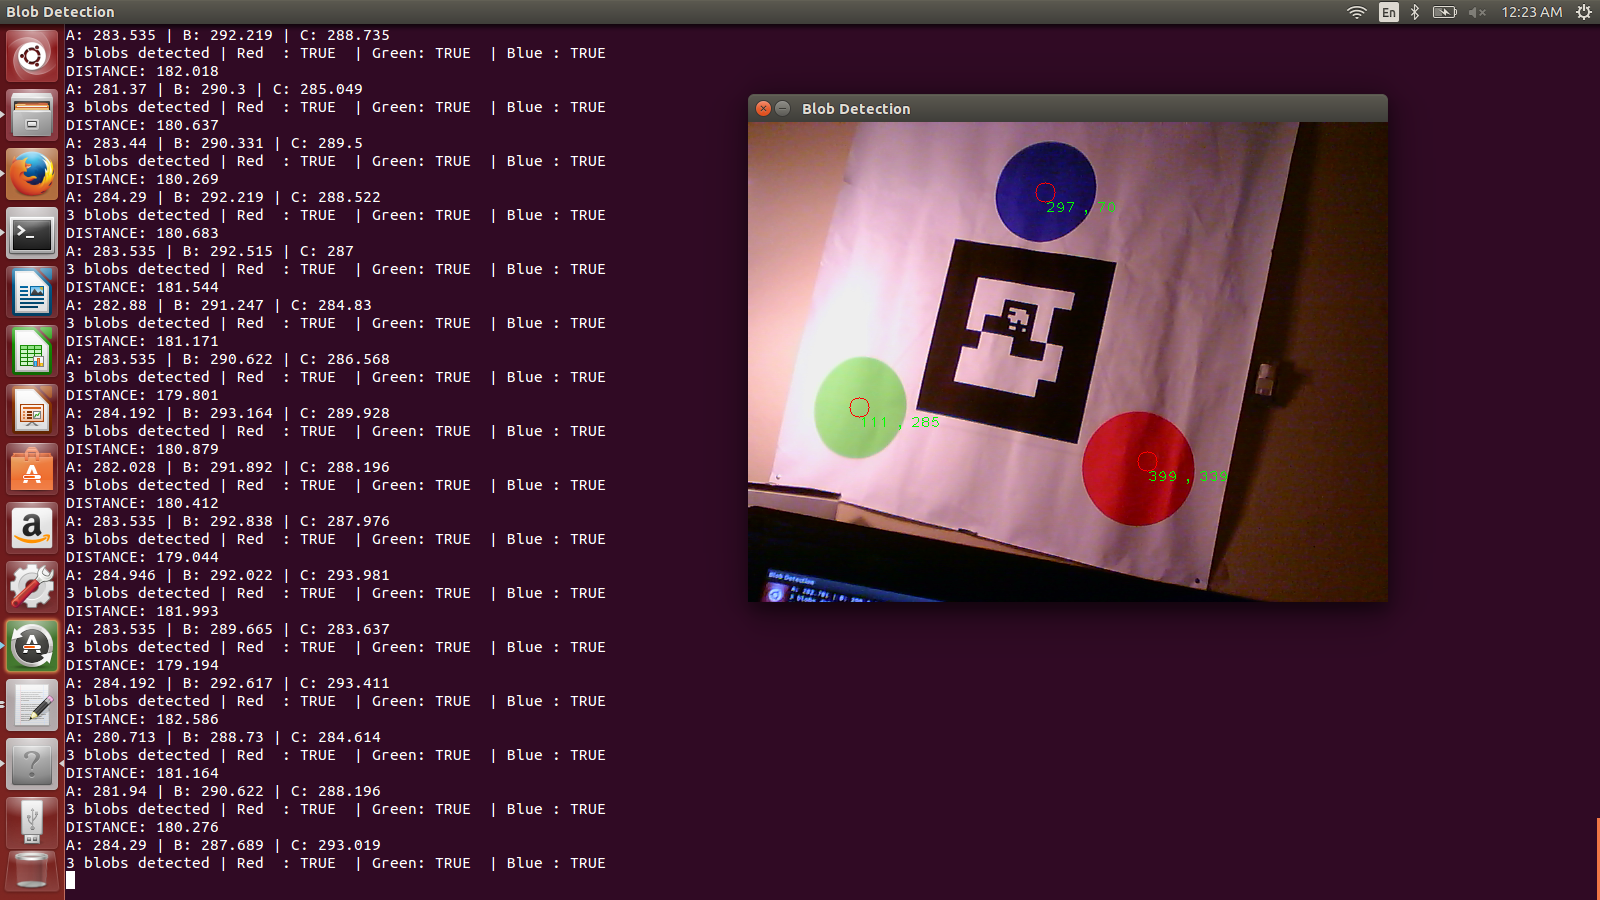
\includegraphics[width=.5\textwidth]{images/coolpic.png} \end{center}

It may be hard to notice, but the text that is currently being displayed in the terminal window shows that there are three blobs detected, exactly one for each color. It is also displaying the range to target, which is correct as far as we can tell.

The next image is what we are going to attempt to use for the next target. It has four colored circles, so we should be able to compute homography more accurately.

\begin{center} 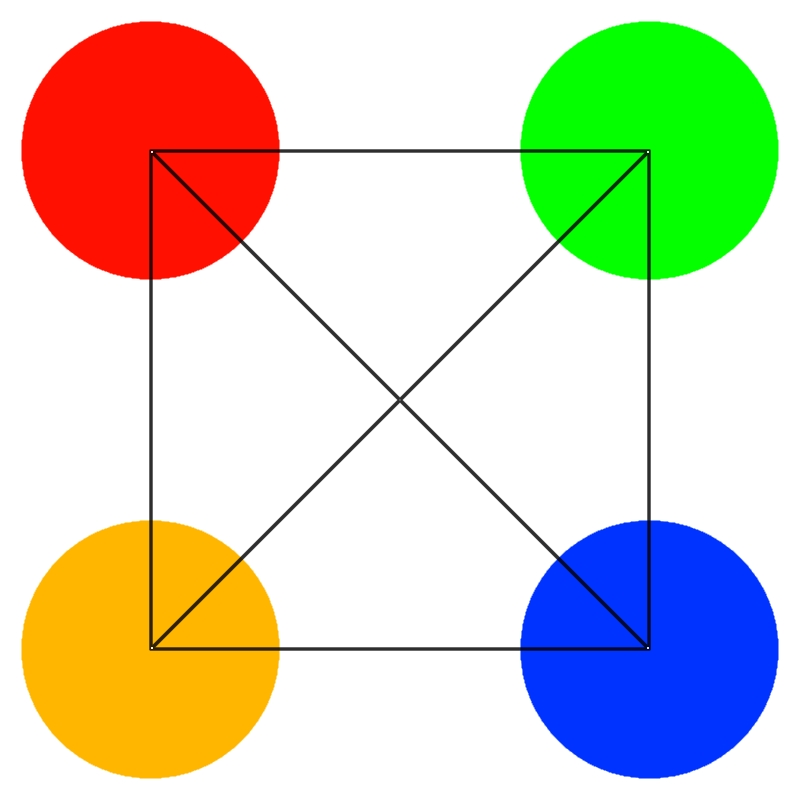
\includegraphics[width=.35\textwidth]{images/landing_guide_small_x.jpg} \end{center}

The final image is just another possible method that we have briefly explored where instead of blob detection we use hough transforms to detect only circles in the images. We have seen papers where others have had successes using targets consisting of concentric circles, so we think that we may be able to have some amount of success with this, in the event that the above methods don't end up panning out.

\begin{center} 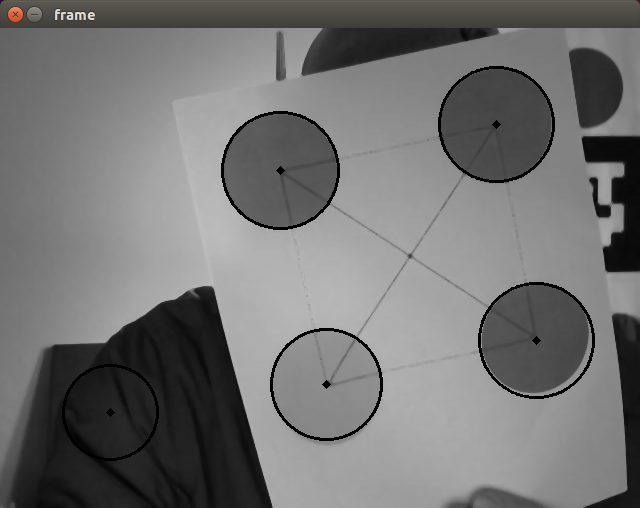
\includegraphics[width=.5\textwidth]{images/circles.png} \end{center}

\subsection{Reinforcement Learning}
\subsubsection{Technologies  Used}
To accomplish the reinforcement learning approach we will be using gazebo and ROS so that we can visually see that the agent is learning the states and actions required to land the UAV.  
\subsubsection{Component  Overview}
\begin{itemize}
  \item Ubuntu 14.04 LTS
  \item Python
  \item C++
  \item ROS pose messages
  \item sarsa\_alg: \\
  \\
  The class that instantiates the agent and performs the appropriate calculations to pick an action to move on to the next state and recieves a reward. Each action will send the appropriate messages to gazebo so that the UAV moves accordingly and allows the user to visually see what the agen is doing.
  \item sarsa\_node: \\
  \\
  The ROS nod that creates the sarsa\_alg class and handles initial topics to publish to and receive from.
\end{itemize}
\subsubsection{Phase Overview}
The Linear, gradient-descent Sarsa($lambda$) with binary features and $\epsilon$-greedy policy will be the algorithm of reinforcement learning that will be implemented. Currently ideas for using a 2-D state space are in the works with a vector field graient to be the actions to funnel the UAV into the center of a cone at a given height and radius. Because of the setbacks of the simulation no coding as been accomplished, but will be as soon as an environment is set up.

\subsubsection{Design Details}
\begin{algorithm} [h]                     % enter the algorithm environment
\caption{Linear, gradient-descent Sarsa($\lambda$) with binary features and $\epsilon$-greedy policy}         
 % give the algorithm a caption
\label{Sarsa}                           % and a label for \ref{} commands later in the document
\begin{algorithmic}                  % enter the algorithmic environment
    \STATE Initialize $\vec{\theta}$ arbitrily and $\vec{e} = \vec{0}$
    \FOR{Each Episode}
      \STATE $s \leftarrow$ initial state of episode
      \FOR{all $a \in A(s)$}
        \STATE $F_a \leftarrow$ set of features present in s, a
        \STATE $Q_a \leftarrow \sum_{i \in F_a}\theta(i)$
      \ENDFOR
      \STATE $a \leftarrow$ arg $max_a Q_a$
      \STATE With probability $\epsilon: a \leftarrow$ a random action $\in A(s)$
      \FOR{ Each Step of Episode}
        \STATE $\vec{e} \leftarrow \gamma \lambda \vec{e}$
        \FOR{ All $\bar{a} \neq a$}
          \FOR{All $i \in F_{\bar{a}}$}
            \STATE $e(i) \leftarrow 0 $
          \ENDFOR
        \ENDFOR
        \FOR{All $i \in F_a$}
          \STATE $e(i) \leftarrow 1 $
        \ENDFOR
        \STATE Take action $a$, observe reward, r, and next state, s'
        \STATE $\delta \leftarrow r - Q_a$
        \FOR{All $a \in A(s')$}
          \STATE $F_a \leftarrow$ set of features present in s', a
          \STATE $Q_a \leftarrow \sum_{i \in F_a}\theta(i)$
        \ENDFOR
        \STATE $a' \leftarrow$ arg $max_a Q_a$
        \STATE With probability $\epsilon:a' \leftarrow$ a random action $\in A(s)$
        \STATE $\delta \leftarrow \delta + \gamma Q_{a'}$
        \STATE $\vec{\theta} \leftarrow \vec{\theta} + \alpha \delta \vec{e}$
        \STATE $a \leftarrow a'$
      \ENDFOR
      \STATE until $s'$ is terminal
    \ENDFOR
\end{algorithmic}
\end{algorithm} 

\subsection{Legacy Code}
\documentclass[11pt]{book}

\usepackage[width=7.0in, height=9.0in, top=1.0in, papersize={8.5in,11in}]{geometry}
\usepackage[pdftex]{graphicx}
%\usepackage{datetime}
\usepackage{anyfontsize}
\usepackage{hyperref}
\usepackage{t1enc}
\usepackage{verbatim}
\usepackage{algorithm}
\usepackage{algorithmic}
\usepackage{framed}
\usepackage{pdfpages}
\usepackage{listings}
\usepackage{upquote}
\definecolor{listinggray}{gray}{0.9}
\definecolor{lbcolor}{rgb}{0.9,0.9,0.9}
\lstset{
backgroundcolor=\color{lbcolor},
    tabsize=4,    
%   rulecolor=,
    language=[GNU]C++,
        basicstyle=\scriptsize,
        upquote=true,
        aboveskip={1.5\baselineskip},
        columns=fixed,
        showstringspaces=false,
        extendedchars=false,
        breaklines=true,
        prebreak = \raisebox{0ex}[0ex][0ex]{\ensuremath{\hookleftarrow}},
        frame=single,
        numbers=left,
        showtabs=false,
        showspaces=false,
        showstringspaces=false,
        identifierstyle=\ttfamily,
        keywordstyle=\color[rgb]{0,0,1},
        commentstyle=\color[rgb]{0.026,0.112,0.095},
        stringstyle=\color[rgb]{0.627,0.126,0.941},
        numberstyle=\color[rgb]{0.205, 0.142, 0.73},
%        \lstdefinestyle{C++}{language=C++,style=numbers}’.
}
\lstset{
    backgroundcolor=\color{lbcolor},
    tabsize=4,
  language=C++,
  captionpos=b,
  tabsize=3,
  frame=lines,
  numbers=left,
  numberstyle=\tiny,
  numbersep=5pt,
  breaklines=true,
  showstringspaces=false,
  basicstyle=\footnotesize,
%  identifierstyle=\color{magenta},
  keywordstyle=\color[rgb]{0,0,1},
  commentstyle=\color{green},
  stringstyle=\color{red}
  }

\pagestyle{empty}
\usepackage{helvet}
\renewcommand{\familydefault}{\sfdefault}
\begin{document}
\section*{Legacy Computer Vision Code}
\noindent The purpose of this section is to document the code from previous years that the team attempted to use for the vision portion of the project. While the team did eventually end up deciding not to take this approach, which involves blob detection, a lot was learned about the process, and if nothing else, we were required to think about the problem of vision much more thoroughly. The code is split up into multiple source files, each file having its own purpose. While this topic is indeed briefly touched upon in the prototypes section of this document, this section will go into much more depth in examining the code, and describing how it functions. The files used are:
\begin{itemize}
\item Camera.h/cpp
\item Coord.h/cpp
\item LED.h/cpp
\item Triangle.h/cpp
\item tracker.cpp
\end{itemize}

\section*{tracker.cpp}
\large{\textbf{Overview}}\\
\normalsize
\noindent The file tracker.cpp contains the main control structure for the blob detection and tracking used by previous teams. Julian Brackins (the original author of the file) provided the following description of the file, which is included in the listing of the contents of the file as well:

\begin{quote}
\centering
This software should hopefully soon be adapted into a ROS publisher that is capable of sending messages to our UAV to indicate the craft's distance from our landing pad situated on our Unmanned Ground Vechicle (UGV). This is done using three equidistant coloured dots, or "blobs" situated on our landing pad. Utilizing OpenCv's libraries for tracking specific colours, these three blobs are recognized by the software's camera feed, with corresponding coordinates in relation to the camera feed's image plane. The software compares these values to the stored points read in from the configuration file in order to compare the observed size of the objects being tracked to the known size of these objects that has been previously calibrated and written to a config file.
\end{quote}


\lstinputlisting{tracker.cpp}


\section*{Camera.h/cpp}
\large{\textbf{Overview}}\\
\normalsize
\noindent The Camera class is used to take an image feed that has three colored blobs detected on it, and calculate the distance to the target, based on the known size of the target. Within Camera.h, you can see that there are a couple of options for the paper size, and these will need to be changed at the time of compilation so that the system will be able to accurately calculate the distance to the target. The method used to calculate the distance to the target is to simply take some known distance to the target that has a pixel width associated with it, and calculate the focal length for the camera. Then, we just divide the focal length by the pixel distance on our measurement and multiply that result by the known width of the target in order to get the new distance.

\[focal\_length = pixel\_width * known\_dist\_to\_target / known\_width\_of\_target \]
\[measured\_dist\_to\_target = known\_width\_of\_target * focal\_length / pixel\_width \]

\large{\textbf{Camera.h}}
\lstinputlisting{Camera.h}
\large{\textbf{Camera.cpp}}
\lstinputlisting{Camera.cpp}

\section*{Coord.h/cpp}
\large{\textbf{Overview}}\\
\normalsize
\noindent The Coord class is used to provide coordinate functionality, which is to say that it will be used by later classes to allow them to store coordinates.

\large{\textbf{Coord.h}}
\lstinputlisting{Coord.h}
\large{\textbf{Coord.cpp}}
\lstinputlisting{Coord.cpp}


\section*{Triangle.h/cpp}
\large{\textbf{Overview}}\\
\normalsize
\noindent The Triangle class is used to allow the program to store a set of three coordinates that make up the triangle of the blobs on the target. The class stores the coordinates of each vertex of the triangle, along with the lengths of each triangle edge. Additionally, it will store the angle between the edges, that can be used to see how "straight on" the image has been taken from.

\large{\textbf{Triangle.h}}
\lstinputlisting{Triangle.h}
\large{\textbf{Triangle.cpp}}
\lstinputlisting{Triangle.cpp}

\section*{LED.h/cpp}
\large{\textbf{Overview}}\\
\normalsize
\noindent The LED class essentially is there to allow definitions of the different colors that are in the blobs being searched for. While the class is named LED, it would be more accurate to rename it to blobs, since detecting colored LEDs was replaced with detecting colored blobs.

\large{\textbf{LED.h}}
\lstinputlisting{LED.h}
\large{\textbf{LED.cpp}}
\lstinputlisting{LED.cpp}


\section*{Final Conclusions About Legacy Code}
\large{\textbf{Functionality}}\\
\normalsize
\noindent Fortunately, the legacy code provided by the 2014-2015 UAV/UGV team is definitely functional. However, due to time constraints, that team was unable to "ROSify" the code by creating a ROS publisher for the data being generated within tracker.cpp. While three blobs being detected should be plenty to determine orientation of and distance to the target, after having members complete the Computer Vision course at school, it was decided that it may be worthwhile to pursue a four-blob approach to allow use of some homography techniques that were used in that course. However, this never ended up turning into anything. Eventually, it was decided that it would be best to use the ROS library AR\_Track\_Alvar, since it is already implemented in ROS, and provides all functionality that would be needed by the team.\\\\
\large{\textbf{Using the Legacy Code}}\\
\normalsize
\noindent It is important to understand how to run this code to see the progress made by previous teams. This provided a huge amount of help to the current team, as we were able to have a jumping off point to begin work from, and understand some approaches that worked well, and some things that maybe didn't work as well. To find instructions on running this code, look to the prototypes section of this document, and find the prototypes for Sprint 2, as that will provide information on building and running this code. 




\end{document}

\newpage
\section{UAV Build}
This section details the physical building of the UAV that will be used in autonomous landing.
\subsection{Technologies  Used}
The technologies that we currently have are listed below and include the controllers required for autonomous flight.
\begin{itemize}
	\item Turnigy Talong V1.0 Hexcopter
	\item 6x DC Motors
	\item 6x Electronic Speed Controllers
	\item 3DR Pixhawk
	\item Odroid-XU4
\end{itemize}
\subsection{Phase Overview}
We are currently in the first phase of UAV construction. In this phase we have completed the construction of the \textbf{Turnigy Talong V1.0 Hexcopter} frame, and mounting all of the DC motors and electronic speed controllers.
\subsection{Design Details}
Current documentation on the build progress made in Sprint 3 is shown below in our BuildProcess.pdf document.
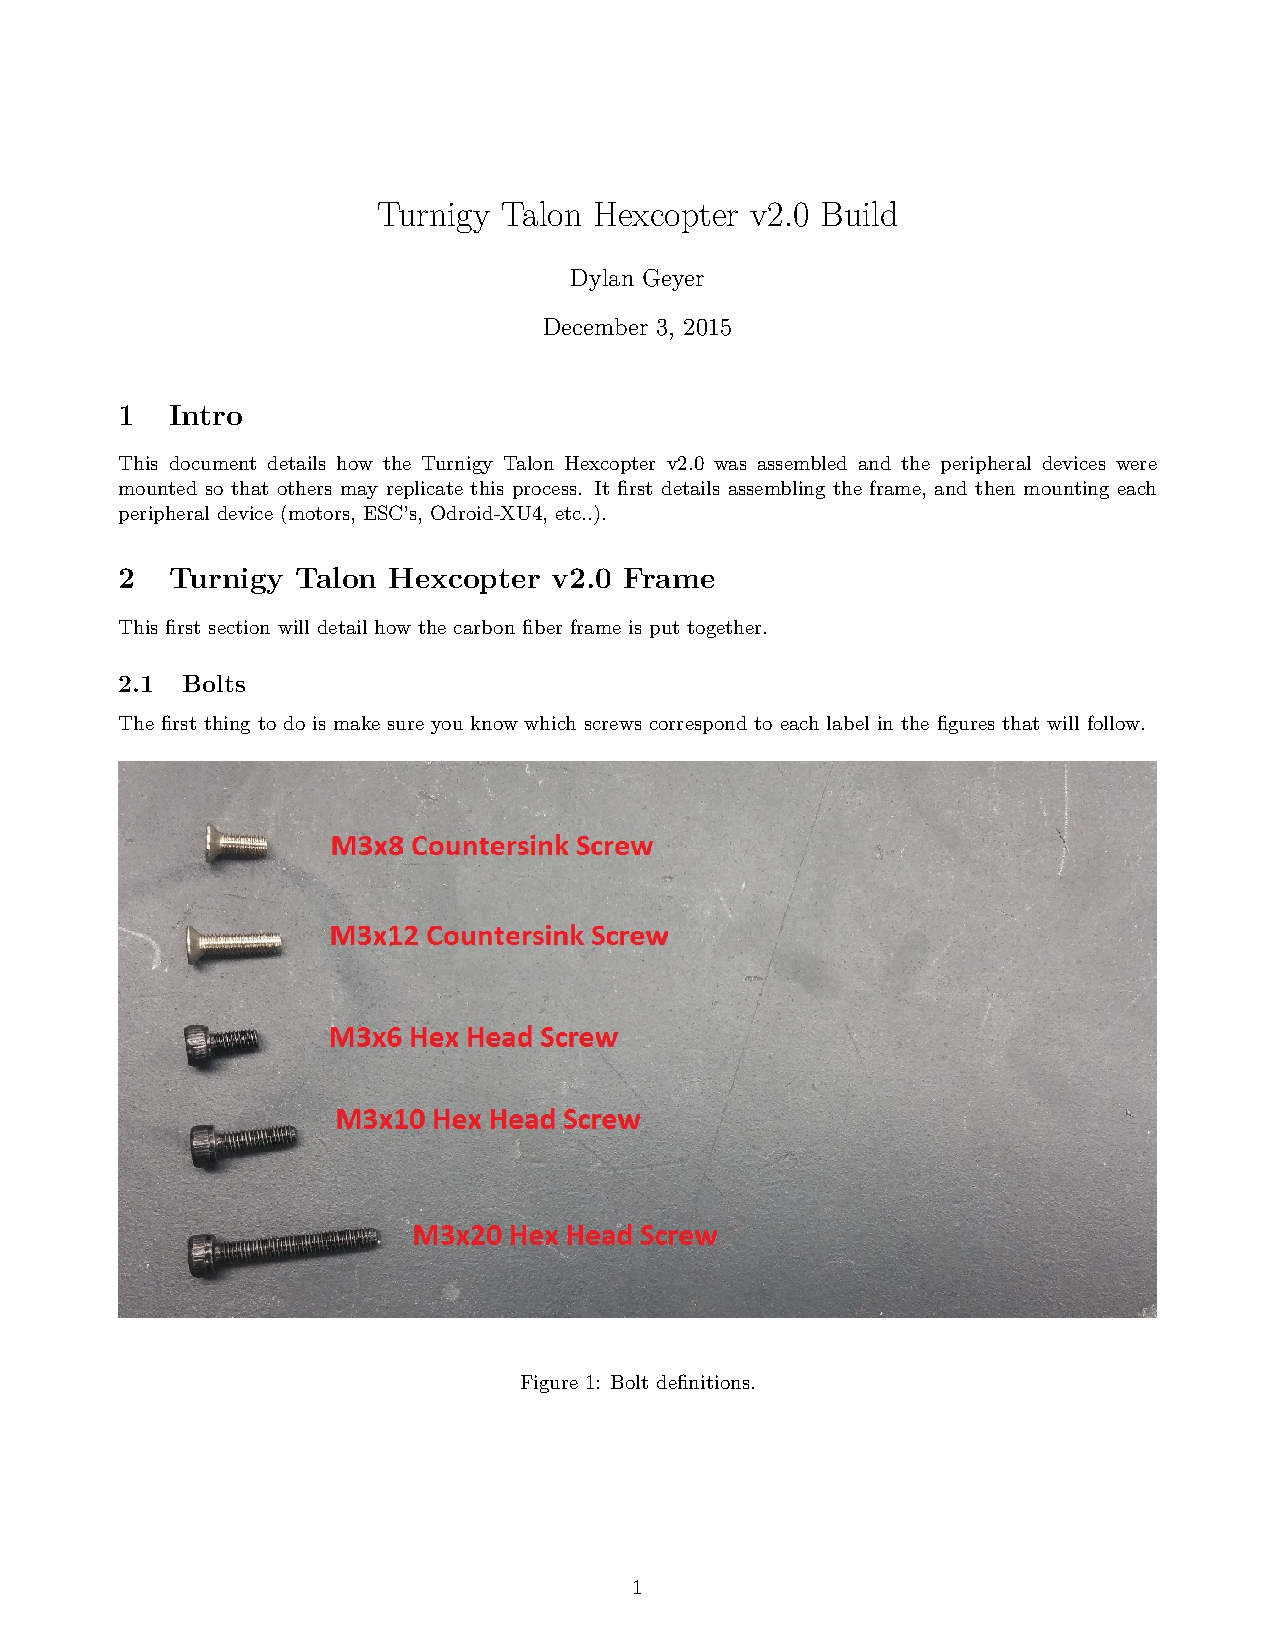
\includepdf[pages={1,2,3,4,5}]{../Documents/Prototypes/Sprint_3/BuildProcedure/BuildProcess.pdf}


%\begin{algorithm} [h]                     % enter the algorithm environment
%\caption{Calculate $y = x^n$}          % give the algorithm a caption
%\label{alg1}                           % and a label for \ref{} commands later in the document
%\begin{algorithmic}                    % enter the algorithmic environment
%    \REQUIRE $n \geq 0 \vee x \neq 0$
%    \ENSURE $y = x^n$
%    \STATE $y \Leftarrow 1$
%    \IF{$n < 0$}
%        \STATE $X \Leftarrow 1 / x$
%        \STATE $N \Leftarrow -n$
%    \ELSE
%        \STATE $X \Leftarrow x$
%        \STATE $N \Leftarrow n$
%    \ENDIF
%    \WHILE{$N \neq 0$}
%        \IF{$N$ is even}
%            \STATE $X \Leftarrow X \times X$
%            \STATE $N \Leftarrow N / 2$
%        \ELSE[$N$ is odd]
%            \STATE $y \Leftarrow y \times X$
%            \STATE $N \Leftarrow N - 1$
%        \ENDIF
%    \ENDWHILE
%\end{algorithmic}
%\end{algorithm} 
 
%\begin{lstlisting}
%#include <stdio.h>
%#define N 10
%/* Block
% * comment */
% 
%int main()
%{
%    int i;
% 
%    // Line comment.
%    puts("Hello world!");
% 
%    for (i = 0; i < N; i++)
%    {
%        puts("LaTeX is also great for programmers!");
%    }
% 
%    return 0;
%}
%\end{lstlisting}
%This code listing is not floating or automatically numbered.  If you want auto-numbering, but it in the algorithm environment (not algorithmic however) shown above.

\newpage
\section{Software: ROS Vision}
This section serves as an overview of the packages used to determine the landing pad, as well as estimate pose, by means of monocular vision. This description will include the packages, launch files, as well as other files needed to implement the AR tag tracking and pose estimation activities. This section is divided into sections covering the different portions of the ROS Vision build, as follows:
\begin{itemize}
\item Camera Operation
\item Camera Calibration
\item Image Processing
\item AR Tag Tracking
\item Pose Estimation
\end{itemize}

\subsection{Camera}
\textbf{usb\_cam}: this ros package provides a method for bringing usb cameras into the ros environment. The node will publish an image topic.

\begin{itemize}
\item License: BSD
\item Documentation: \url{http://wiki.ros.org/usb_cam}
\item Source: \url{https://github.com/bosch-ros-pkg/usb_cam}
\item Parameters
\begin{itemize}
\item image width: pixel width. Default: 640\\
\textit{param data type}: integer
\item image height: pixel height. Default: 480\\
\textit{param data type}: integer
\item pixel\_format: mjpeg, yuyv, or uyvy. Default: mjpeg\\
\textit{param data type}: string
\item io\_method: mmap, read, or userptr. Default: mmap\\
\textit{param data type}: string
\item camera\_frame\_id: name of the camera tf frame. Default: head\_camera\\
\textit{param data type}: string
\item framerate: framerate of the camera. Default: 30\\
\textit{param data type}: integer
\item contrast: contrast of the image (integer value [0-255]). Default: 32\\
\textit{param data type}: integer
\item brightness: brightness of the image (integer value [0-255]). Default: 32\\
\textit{param data type}: integer
\item saturation: saturation of the image (integer value [0-255]). Default: 32\\
\textit{param data type}: integer
\item sharpness: sharpness of the image (integer value [0-255]). Default: 22\\
\textit{param data type}: integer
\item autofocus: enable/disable autofocus. Default: False.\\
\textit{param data type}: boolean
\item camera\_info\_url: string value of url of calibration file.\\
\textit{param data type}: string
\item camera\_name: the camera name, which must match the name in the calibration file.\\
\textit{param data type}: string
\end{itemize}
\item Published Topics
\begin{itemize}
\item /image - containing the sensor\_msgs/Image message
\end{itemize}
\item Installation:
\begin{lstlisting}[language=bash]
$ sudo apt-get-install ros-jade-usb-cam
\end{lstlisting}
\item Sample Launch File
\lstset{language=XML}
\begin{lstlisting}
<launch>
	<node pkg="usb_cam" type="usb_cam_node" name="usb_cam">
		<param name="video_device" type="string" value="/dev/video0"/>
		<param name="image_width" type="int" value="640" />
		<param name="image_height" type="int" value="480" />
		<param name="pixel_format" type="string" value="yuyv"/>
		<param name="camera_frame_id" value="camera" />
	</node>
</launch>
\end{lstlisting}
\end{itemize}



 
\noindent \textbf{pointgrey\_camera\_driver}: this ros package provides a method for bringing point grey cameras into the ros environment. 

\begin{itemize}
\item License: BSD
\item Documentation: \url{http://wiki.ros.org/pointgrey_camera_driver}
\item Source: \url{https://github.com/ros-drivers/pointgrey_camera_driver}
\item Parameters
\begin{itemize}
\item video\_mode: There are several types supported by the driver. It is important the correct one is used. 
\begin{itemize}
\item use "Format0\_Mode5" for video mode 640x480\_mono8
\item use "Format0\_Mode6" for video mode 640x480\_mono16
\item use "Format2\_Mode1" for video mode 1280x960\_bayer8
\item use "Format2\_Mode2" for video mode 1280x960\_mono8
\item use "Format2\_Mode6" for video mode 1280x960\_mono16
\item use "Format7\_Mode0" for video mode format7\_mode0
\item use "Format7\_Mode1" for video mode format7\_mode1
\item use "Format7\_Mode2" for video mode format7\_mode2
\item use "Format7\_Mode3" for video mode format7\_mode3
\end{itemize} 
\textit{param data type}: string

\item frame\_rate:  the camera speed in frames per second \\
\textit{param data type}: double

\item auto\_exposure:  allow the camera to automatically change exposure (Combined Gain, Iris \& Shutter control).\\
\textit{param data type}: boolean

\item exposure: similar to contrast (use double, instead of integer).\\
\textit{param data type}: double

\item auto\_shutter: enable/disable auto shutter\\
\textit{param data type}: boolean
\item shutter\_speed: the time (in seconds) aperture remains open\\
\textit{param data type}: double
\item auto\_gain: emable/disable auto gain\\
\textit{param data type}: boolean
\item gain: set the relative circuit gain\\
\textit{param data type}: double
\item pan: control camera pan\\
\textit{param data type}: integer
\item tilt: control camera tilt\\
\textit{param data type}: integer
\item brightness: set the black level offset\\
\textit{param data type}: double
\item gamma: set the gamma expansion exponent\\
\textit{param data type}: double
\item auto\_white\_balance: enable/disable automatic white balancing. Default: True\\
\textit{param data type}: boolean
\item white\_balance\_blue: set the blue component of white balance\\
\textit{param data type}: integer
\item white\_balance\_red: set the red component of white balance\\
\textit{param data type}: integer
\item format7\_roi\_width: width of Format7 Region of Interest in unbinned pixels, full width if zero \\
\textit{param data type}: integer
\item format7\_roi\_height: height of Format7 Region of Interest in unbinned pixels, full height if zero\\
\textit{param data type}: integer
\item format7\_x\_offset: horizontal offset for left side of Format7 ROI in unbinned pixels\\
\textit{param data type}: integer
\item format7\_y\_offset: Vertical offset for top of Format7 ROI in unbinned pixels\\
\textit{param data type}: integer
\item format7\_color\_coding: Only use if using Format7 modes
\begin{itemize}
\item use "Mono8" for color coding format mono8
\item use "Mono16" for color coding format mono16
\item use "Raw8" for color coding format raw8
\item use "Raw16" for color coding format raw16
\end{itemize}
\textit{param data type}: string
\end{itemize}
\item Published Topics
\begin{itemize}
\item <camera>/image\_raw - the image file
\item <camera>/camera\_info - information from the calibration file
\end{itemize}
\item Installation: 
\begin{lstlisting}[language=bash]
$ sudo apt-get install ros-jade-pointgrey-camera-driver
\end{lstlisting}
\item Sample Launch File
\lstset{language=XML}
\begin{lstlisting}
<launch>
   <!-- Determine this using rosrun pointgrey_camera_driver list_cameras.
       If not specified, defaults to first camera found. -->
  <arg name="camera_serial" default="0" />
  <arg name="calibrated" default="0" />

  <group ns="camera">
    <node pkg="nodelet" type="nodelet" name="camera_nodelet_manager" 
     args="manager" />

    <node pkg="nodelet" type="nodelet" name="camera_nodelet"
          args="load pointgrey_camera_driver/PointGreyCameraNodelet 
                camera_nodelet_manager" >
      <param name="frame_id" value="camera" />
      <param name="serial" value="$(arg camera_serial)" />

      <!-- When unspecified, the driver will use the default framerate 
           as given by the camera itself. Use this parameter to override
           that value for cameras capable of other framerates. -->
      <!-- <param name="frame_rate" value="15" /> -->
      
      <!-- Use the camera_calibration package to create this file -->
      <param name="camera_info_url" if="$(arg calibrated)"
             value="file://$(env HOME)/.ros/camera_info/
                    $(arg camera_serial).yaml" />
    </node>

    <node pkg="nodelet" type="nodelet" name="image_proc_debayer"
          args="load image_proc/debayer camera_nodelet_manager">
    </node>
  </group>
</launch>
\end{lstlisting}
NOTE: This launch file is THE launch file provided by the repository, and will be available when you install this package. A few notes about what is occuring in this file before we go any further. The call for a camera calibration file will become clear in the next subsection. Additionally, this launch file is somewhat complicated by the use of nodelets which is a thing in ROS designed to reduce the complexity of the node networks in terms of communication. In the words of the ROS deities at \href{http://www.clearpathrobotics.com/guides/ros/Nodelet%20Everything.html}{Clear Path Robotics}
\begin{quotation}
The primary advantage is the automagic zero-copy transport between nodelets (in one nodelet manager). This means that the pointcloud created by a hardware driver doesn’t need to get copied or serialized before it hits your code, assuming you inject the nodelet into the camera’s manager, saving you time and trouble.

You get all the modularity of nodes, and all the efficiency of having one monolithic process. This makes nodelets more flexible than bare plugins (via pluginlib) - you can implicitly tap into any of the intra-process communication that occurs.
\end{quotation}
We leave it to the reader to learn more about nodelets should that be a path that appears to offer substantial benefit. The team made modifications to this file that will be discussed in a later subsection.
\end{itemize}

\subsection{Camera Calibration}
\noindent \textbf{camera\_calibration}: This package is used to calibrate both monocular and stereo cameras. The package has two functions, camera calibration and camera check. Camera check is to check the calibration of the camera. This may be a good idea to use after calibration is performed as an extra measure to ensure a good calibration was made by the calibration step.\\ 

\noindent Before starting, it is necessary to get a calibration board. For this calibration, a chess board image is required. The interior corner count and size of chess board square in meters is needed. A sample board is shown in the figure HERE below. This board can be found \href{http://wiki.ros.org/camera_calibration/Tutorials/
MonocularCalibration?action=AttachFile&do=view&target=check-108.pdf}{here}. This board is a 6 $\times$ 8 board (count the interior corners of the squares along the width and height, you should get 6 and 8). Be sure to measure a square after printing in meters and use that value in the call to run this package.\\ 

\begin{itemize}
\item License: BSD
\item Documentation: \url{http://wiki.ros.org/camera_calibration}
\item Source: \url{https://github.com/ros-perception/image_pipeline}
\item Subscribed Topics
\begin{itemize}
\item image: this is the image being published by the respective camera 
\item camera: this is the camera topic being published by the respective camera
\end{itemize}
\item Installation:
\begin{lstlisting}[language=bash]
$ sudo apt-get install ros-jade-camera-calibration
\end{lstlisting}
\item Usage:
\begin{enumerate}
\item start camera in ROS environment
\item begin camera calibration by using the following sample command, which has been modified for a board printed on standard A4 paper. (\href{http://wiki.ros.org/camera_calibration}{the original sample is found at the package documentation site}):
\begin{lstlisting}[language=bash]
$ rosrun camera_calibration cameracalibrator.py --size 8x6 --square 0.0254 image:=/camera/raw_image camera:=/camera
\end{lstlisting}
\item A window will open containing an image like that in figure ~\ref{calib}. It is important to move the chess board about traversing the frame near and distant, and about the extremes of the image frame. It is VERY important to be slow and deliberate with your movements while calibrating. Quick jerky movements will still result in a valid calibration, but the calibration may not be accurate enough when it comes time to track the AR tag or use this information for visual odometry, discussed later in the localization subsection.\\
\begin{figure}[h]
\caption{Example of calibrating the camera}
\centering
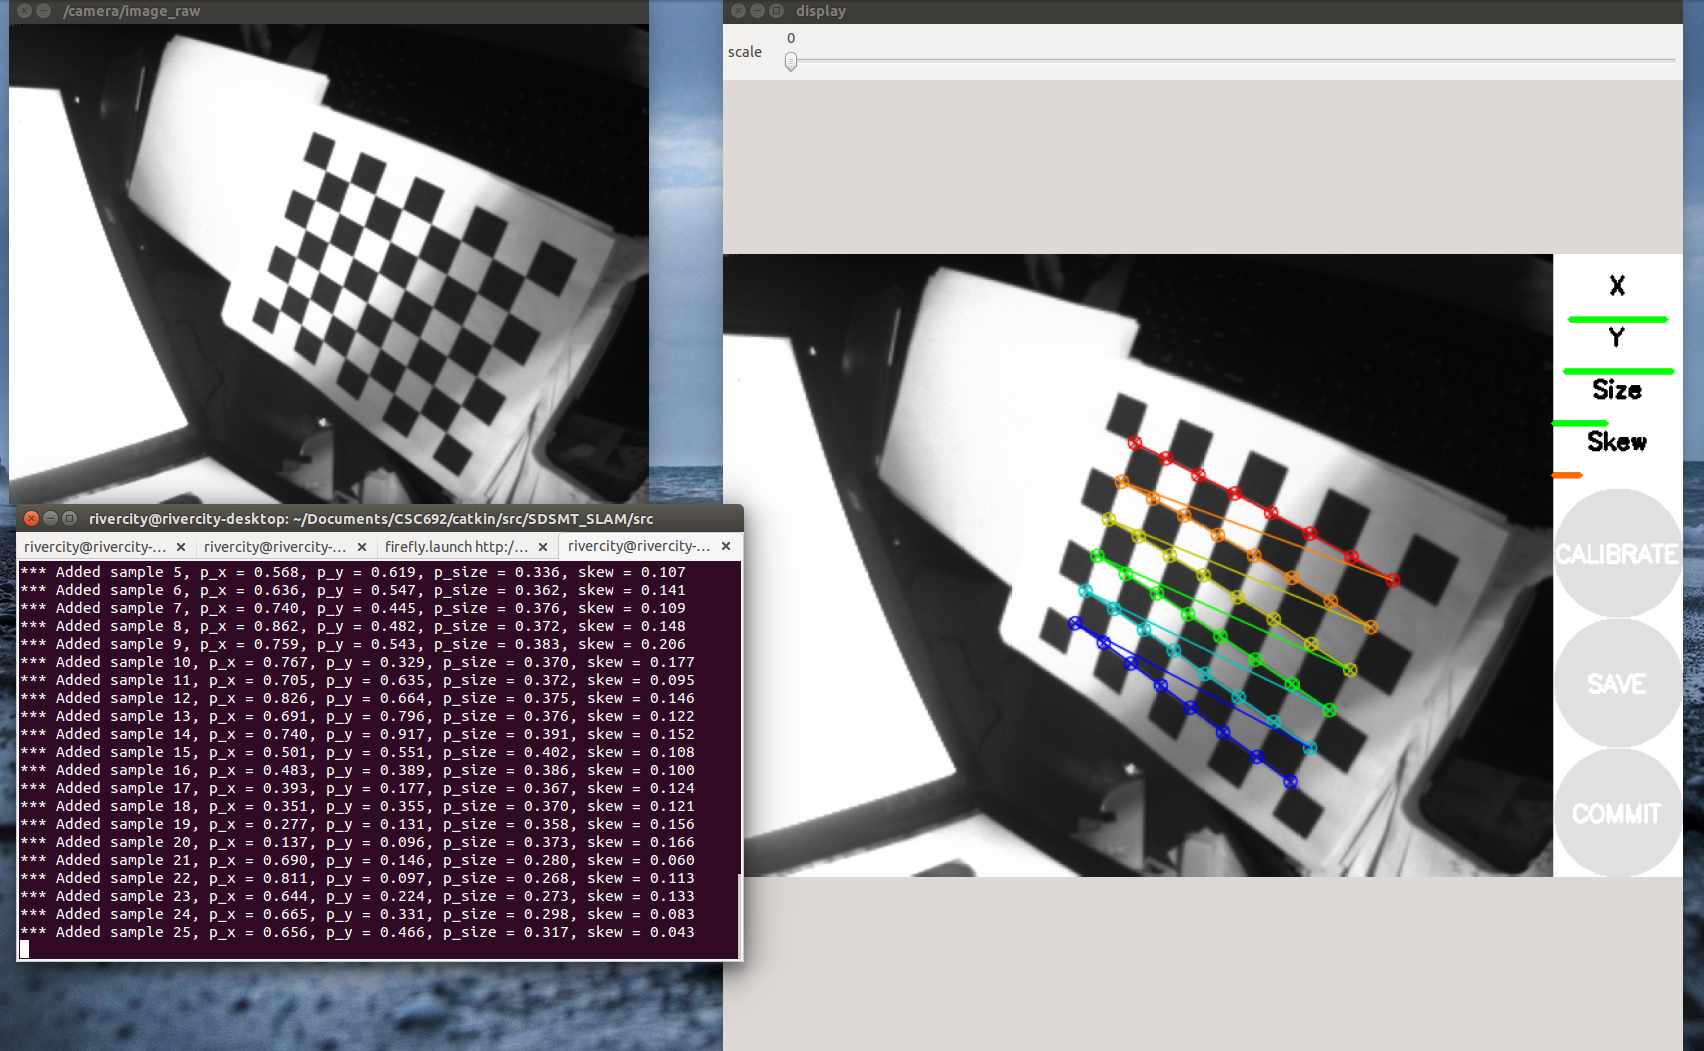
\includegraphics[width=.75\textwidth]{images/calibration}
\label{calib}
\end{figure}
As a note, figure ~\ref{calib_graph} is a useful example of the calibration with the firefly camera. Both firefly and and webcam calibrations will necessitate the subscription of the raw image by the calibration package. The camera\_info topic is useless here, because we are trying to discover the calibration, and so we only want the raw image, and the output will be the calibration file.\\
\begin{figure}[h]
\caption{Graph of ROS topics during calibration}
\centering
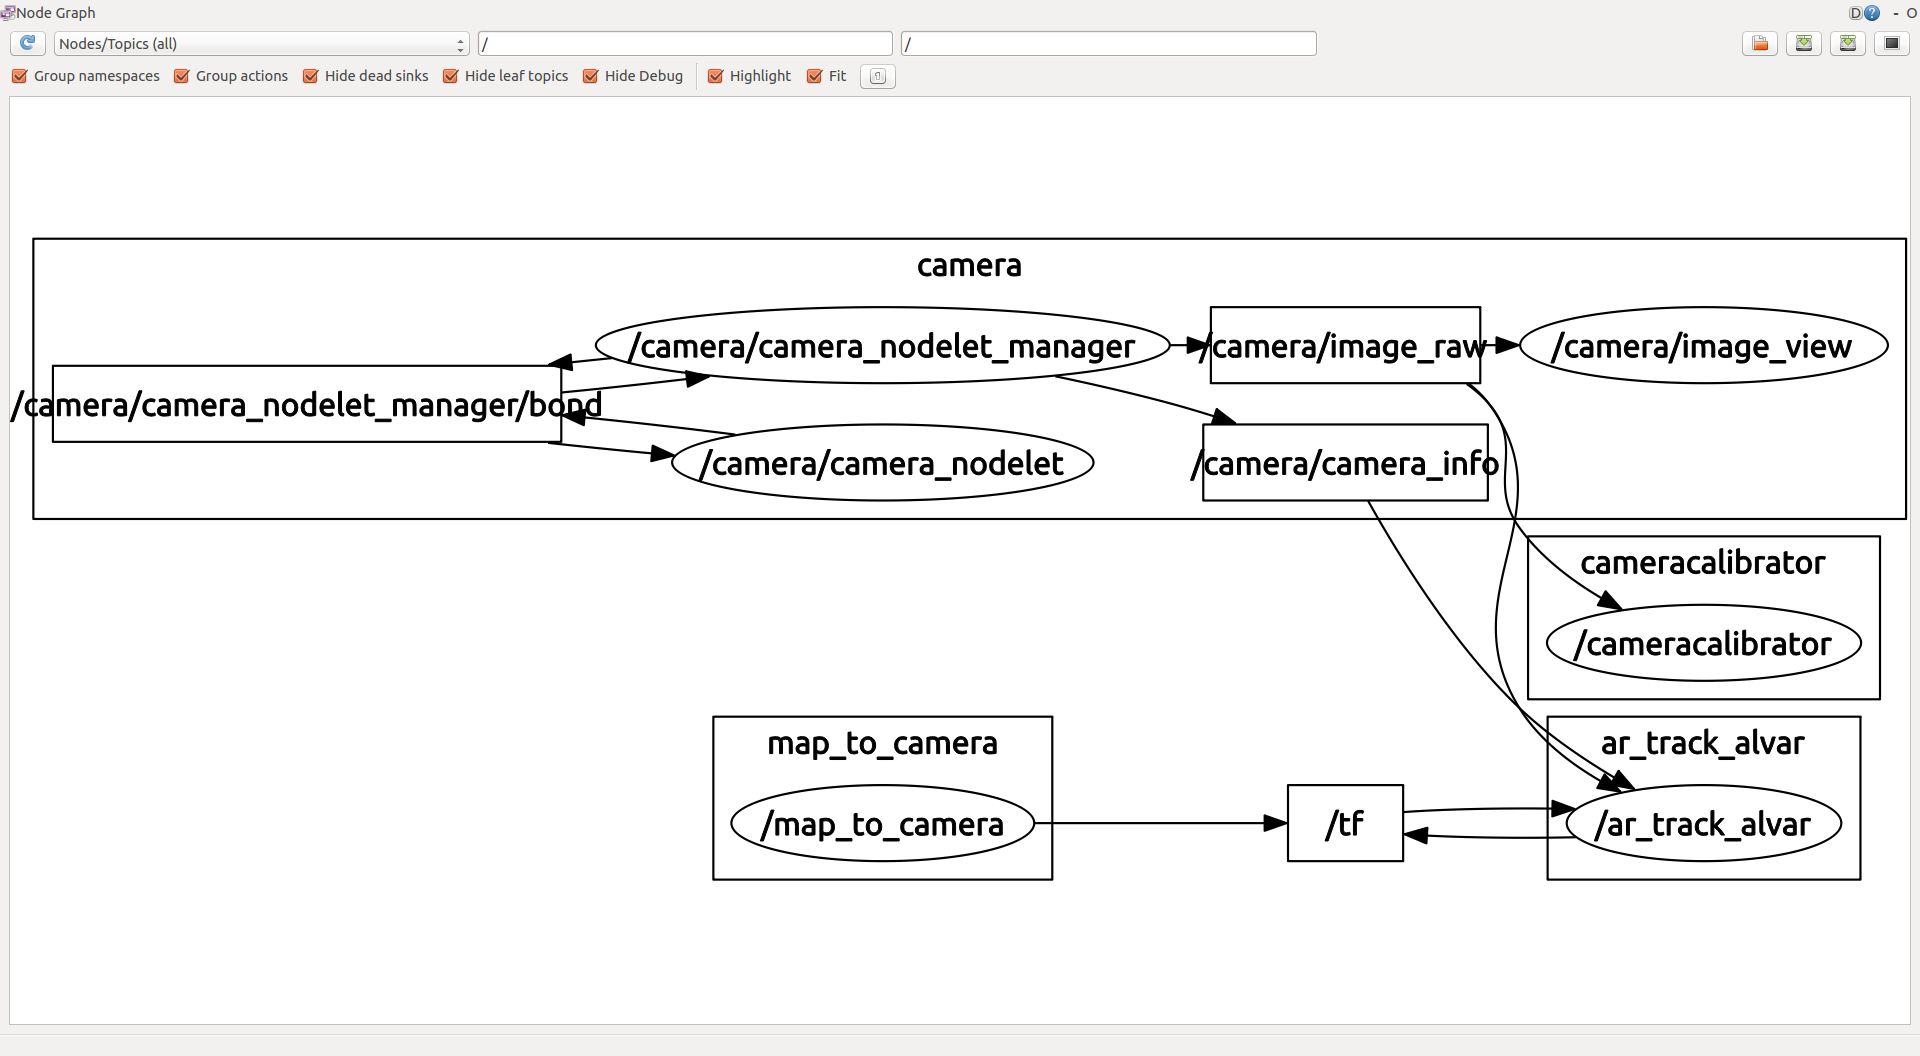
\includegraphics[width=.75\textwidth]{images/calib_graph}
\label{calib_graph}
\end{figure}
\item After the calibration is complete, the file will be saved to in the ros camera calibration file found by navigating to:
\begin{lstlisting}[language=bash]
$ cd ~/.ros/camera_info
\end{lstlisting}

A quick peek into this directory will reveal, yaml files for the calibrated camera.
\begin{lstlisting}[language=bash]
$ ls
0.yaml	head_camera.yaml
\end{lstlisting}
In this example, the firefly and webcam have both been calibrated, represented by the 0.yaml and head\_camera.yaml files respectively.\\

This calibration will be used by the tag tracking directly, and there will some changes that will need to be made to make it usable. That will be covered in the localization section. However, it is very important to understand where this file is located. You can change this location, but the parameter in the launch file will need to be altered as well to ensure that the package can find the calibration file for reference. Note in the image file we can see that camera name, image dimensions, camera matrix, and distortion coefficients. These become very, very important later on.
%YAML not supported by listings, python best surrogate
\begin{lstlisting}[language=python] 
image_width: 640
image_height: 480
camera_name: head_camera
camera_matrix:
  rows: 3
  cols: 3
  data: [974.876804668264, 0, 310.0364238884084, 0, 977.9747558767541, 183.9139863795955, 0, 0, 1]
distortion_model: plumb_bob
distortion_coefficients:
  rows: 1
  cols: 5
  data: [-0.09363555823455676, -0.1141346935352986, -0.008866235140581833, -0.0048644735641969, 0]
rectification_matrix:
  rows: 3
  cols: 3
  data: [1, 0, 0, 0, 1, 0, 0, 0, 1]
projection_matrix:
  rows: 3
  cols: 4
  data: [962.1740112304688, 0, 307.6517383159608, 0, 0, 965.6265258789062, 181.2353823390822, 0, 0, 0, 1, 0]
\end{lstlisting}
\end{enumerate}
\end{itemize}

\subsection{Image Processing}
\noindent \textbf{image\_proc}: This package is necessary for color cameras, as the svo step requires the use of grayscale images. This package provides a number of convenient tools in addition to translating color to grayscale. The images can also be rectified through this tool. However, for the purpose of this project, it is important that the launch file is NOT configured to do this. Doing so will result in calibration being applied twice, which will result in a distorted image.\\

\begin{itemize}
\item License: BSD
\item Documentation: \url{http://wiki.ros.org/image_proc}
\item Source: \url{https://github.com/ros-perception/image_pipeline}
\item Parameters
\begin{itemize}
\item queue\_size: message queue for synchronizing image and camera\_info topics. May need adjustment if camera\_info is coming much faster than image\_raw messages. Default: 5\\
\textit{param data type}: integer
\item decimation\_x: the number of pixels to decimate to one horizontally. Range: [1-16]. Default: 1\\
\textit{param data type}: integer
\item decimation\_y: the number of pixels to decimate to one vertically. Range: [1, 16]. Default: 1 \\
\textit{param data type}: integer
\item x\_offset: X offset of the region of interest. Range: [0-2447]. Default: 0 \\
\textit{param data type}: integer
\item y\_offset: Y offset of the region of interest. Range: [0-2049]. Default: 0\\
\textit{param data type}: integer
\item width: width of the region of interest. Range: [0-2448]. Default: 0\\
\textit{param data type}: integer
\item height: height offset of the region of interest. Range: [0-2050]. Default: 0\\
\textit{param data type}: integer
\item interpolation:
\begin{itemize}
\item Nearest-neighbor sampling. Value = 0 
\item Bilinear interpolation. Value = 1 
\item Bicubic interpolation over 4x4 neighborhood. Value = 2
\item Resampling using pixel area relation. Value = 3
\item Lanczos interpolation over 8x8 neighborhood. Value = 4
\end{itemize}
\textit{param data type}: integer
\end{itemize}
\item Subscribed Topics
\begin{itemize}
\item <camera\_topic\_node>/image\_raw: image frames from camera
\item <camera\_topic\_node>/camera\_info: camera metadata from respective calibration file
\end{itemize}
\item Published Topics
\begin{itemize}
\item <camera\_topic\_node>/image\_raw: adjusted output image
\item <camera\_topic\_node>/camera\_info: adjusted camera metadata
\end{itemize}
\item Installation: 
\begin{lstlisting}[language=bash]
$ sudo apt-get install ros-jade-image-proc
\end{lstlisting}
\item Sample Launch File:
\begin{lstlisting}[language=xml]
<launch>
    <node pkg="usb_cam" type="usb_cam_node" name="usb_cam">
        <param name="video_device" type="string" value="/dev/video0"/>
        <param name="image_width" type="int" value="640" />
        <param name="image_height" type="int" value="480" />
        <param name="pixel_format" type="string" value="yuyv"/>
        <param name="camera_frame_id" value="camera" />
    </node>

    <node name="proc" pkg="image_proc" type="image_proc" args="">
        <remap from="image_raw" to="usb_cam/image_raw"/>
        <remap from="camera_info" to="usb_cam/camera_info"/>
    </node>
</launch>
\end{lstlisting}
It may be useful here to explain the remap function. Looking at figure ~\ref{image_proc}, we see the grayscale tranformed image from the color image. When the camera package is advertising the topic, the topic advertised will be coming from its parent node. The processing node, seen in the middle of figure ~\ref{image_proc} won't find image\_raw without a little help. Thus, we remap the topic the processing node is looking for from image\_raw to usb\_cam/image\_raw. So, remap does nothing more than tell the node to subscribe to the topic using a different name.
\begin{figure}[h]
\caption{Grayscale transform of image stream}
\centering
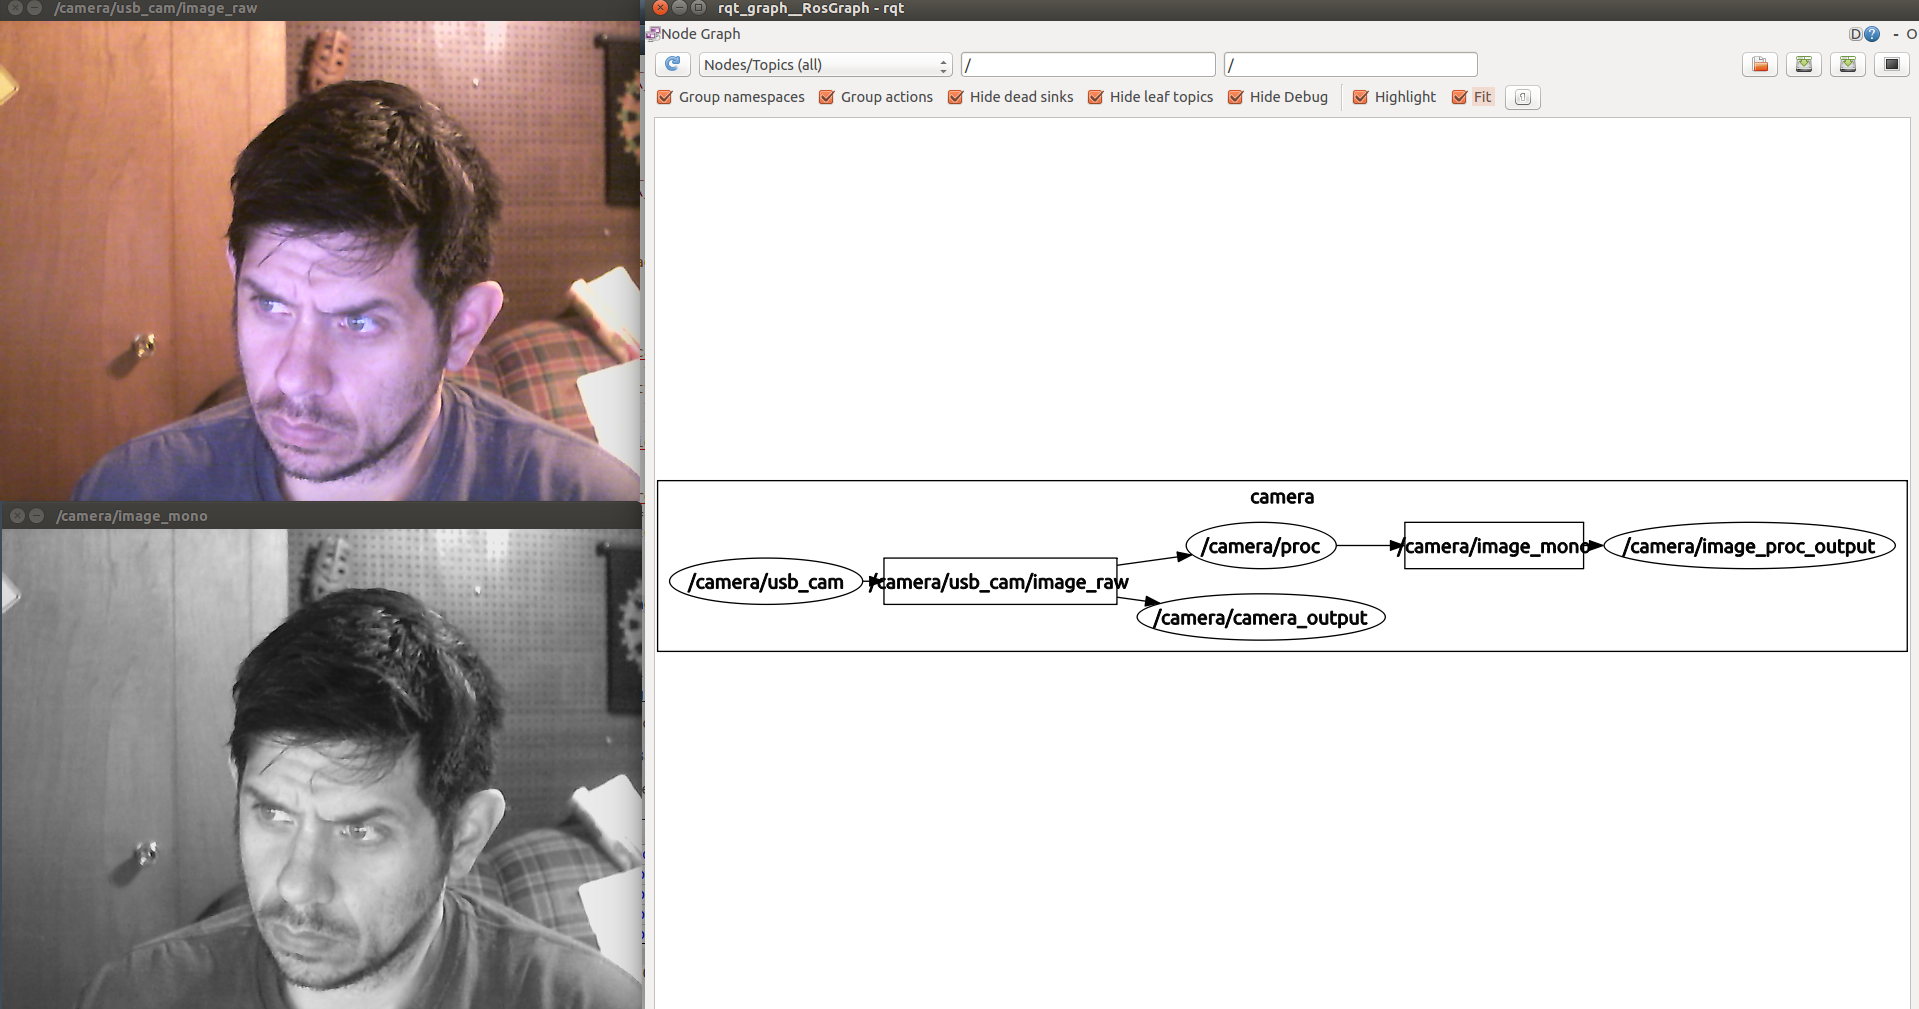
\includegraphics[width=.75\textwidth]{images/image_proc}
\label{image_proc}
\end{figure} 
\end{itemize}

\subsection{Tag Tracking}
\noindent \textbf{ar\_track\_alvar}: this package tracks ar tags in the image frame and performs the visual homography necessary to calculate the distance and orientation of the tag in reference to the camera. It is capable of tracking multiple tags, however, we only need it to track one. Another nice feature of this package is that it will identify the tag being observed. This may be advantageous in later iterations if there are multiple UAVs requiring multiple landing pads.\\

\begin{itemize}
\item License: LGPL-2.1
\item Documentation: \url{http://wiki.ros.org/ar_track_alvar}
\item Source: \url{https://github.com/sniekum/ar_track_alvar}
\item Parameters
\begin{itemize}
\item enabled: enable/disable tracking, unsubscribing from camera topic to stop openni processing. Default: True\\
\textit{param data type}: boolean
\item max\_frequency: maximum processing rate; frames coming at a higher rate are discarded. Range: [1.0-30.0]. Default: 10.0\\
\textit{param data type}: double
\item marker\_size: the width in centimeters of one side of the black square marker border. Range: [1.0-100.0]. Default: 10.0\\
\textit{param data type}: double
\item max\_new\_marker\_error: threshold determining when new markers can be detected under uncertainty. Range: [0.0-2.0]. Default: 0.08\\
\textit{param data type}: double
\item max\_track\_error: threshold determining how much tracking error can be observed before an tag is considered to have disappeared. Range: [0.0-4.0]. Default: 0.2\\
\textit{param data type}: double
\end{itemize}
\item Subscribed Topics
\begin{itemize}
\item <camera\_topic\_node>/image\_raw: image frames from camera
\item <camera\_topic\_node>/camera\_info: camera metadata from respective calibration file
\end{itemize}
\item Published Topics
\begin{itemize}
\item /ar\_pose\_marker: used in rviz for visualization. A colored square will be displayed at the location of the tag.
\item /visualization\_marker: pose information of the AR tag with respect to the output frame.
\end{itemize}
\item Installation:
\begin{lstlisting}[language=bash]
$ sudo apt-get install ros-indigo-ar-track-alvar
\end{lstlisting}
\item Sample Launch File:
\begin{lstlisting}[language=xml]
<launch>
   <!-- Determine this using rosrun pointgrey_camera_driver list_cameras.
       If not specified, defaults to first camera found. -->
  <arg name="camera_serial" default="0" />
  <arg name="calibrated" default="0" />

  <node pkg="tf" type="static_transform_publisher" name="map_to_camera" output="screen" args="0 0 0 0 0 0 world camera 10" />

  <group ns="camera">
      <node pkg="nodelet" type="nodelet" name="camera_nodelet_manager" args="manager" />

      <node pkg="nodelet" type="nodelet" name="camera_nodelet"
            args="load pointgrey_camera_driver/PointGreyCameraNodelet camera_nodelet_manager" >
        <param name="frame_id" value="camera" />
        <param name="serial" value="$(arg camera_serial)" />
        <param name="video_mode" type="string" value="Format0_Mode5"/>
        <param name="frame_rate" type="double" value="70" />
        <param name="shutter_speed" type="double" value="0.00005"/>

        <!-- When unspecified, the driver will use the default framerate as given by the
             camera itself. Use this parameter to override that value for cameras capable of
             other framerates. -->
        <!-- <param name="frame_rate" value="15" /> -->
        
        <!-- Use the camera_calibration package to create this file -->
        <param name="camera_info_url" if="$(arg calibrated)"
               value="file://$(env HOME)/.ros/camera_info/$(arg camera_serial).yaml" />
      </node>

      <node name="image_view" pkg="image_view" type="image_view" respawn="false" output="screen">
        <remap from="image" to="image_raw" />
        <param name="autosize" value="true" />
      </node>
  </group>
 
  <arg name="marker_size" default="12.7" />
  <arg name="max_freq" default="10.0" />
  <arg name="max_new_marker_error" default="0.08" />
  <arg name="max_track_error" default="0.2" />
  <arg name="cam_image_topic" default="/camera/image_raw" />
  <arg name="cam_info_topic" default="/camera/camera_info" /> 
  <arg name="output_frame" default="/camera" />
   
  <node name="ar_track_alvar" pkg="ar_track_alvar" type="individualMarkersNoKinect" respawn="false" output="screen" args="$(arg marker_size) $(arg max_new_marker_error) $(arg max_track_error) $(arg cam_image_topic) $(arg cam_info_topic) $(arg output_frame) 30" />
  

 </launch>
\end{lstlisting}
Above we see many of the previous packages discussed wrapped up into a single launch file along with ar\_track\_alvar. Looking solely at what is needed to call this package we can see in the snippet below from the launch file. Without an image topic and camera\_info topic being actively published, the package will be unable to calculate any type of detect any tag. 

\begin{lstlisting}[language=xml]
  <arg name="marker_size" default="12.7" />
  <arg name="max_freq" default="10.0" />
  <arg name="max_new_marker_error" default="0.08" />
  <arg name="max_track_error" default="0.2" />
  <arg name="cam_image_topic" default="/camera/image_raw" />
  <arg name="cam_info_topic" default="/camera/camera_info" /> 
  <arg name="output_frame" default="/camera" />
   
  <node name="ar_track_alvar" pkg="ar_track_alvar" type="individualMarkersNoKinect" respawn="false" output="screen" args="$(arg marker_size) $(arg max_new_marker_error) $(arg max_track_error) $(arg cam_image_topic) $(arg cam_info_topic) $(arg output_frame) 30" />
\end{lstlisting}
It is crucial that these are set correctly, such as marker\_size, which will determine the distance of the tag from the camera based on that size.\\

This other bit below is a way to instantiate a window to view our camera output image. This is very helpful when attempting to gain pose information as feedback, as image view will let us view our target frame and include the AR tag.
\begin{lstlisting}[language=xml]
      <node name="image_view" pkg="image_view" type="image_view" respawn="false" output="screen">
        <remap from="image" to="image_raw" />
        <param name="autosize" value="true" />
      </node>
\end{lstlisting}

To gain a fantastic visualization of our pose information within the image frame we can call rviz.
\begin{lstlisting}[language=bash]
$ rosrun rviz rviz
\end{lstlisting}
After calling rviz, we need to change our frame to that of our camera. Then we can add the camera, TF, and marker by using the add buttons in rviz and selecting those topics to visualize. The result should be similar to what we see in in figure ~\ref{tracker}.\\
\begin{figure}[h]
\caption{Visualization of ar\_track\_alvar using Rviz}
\centering
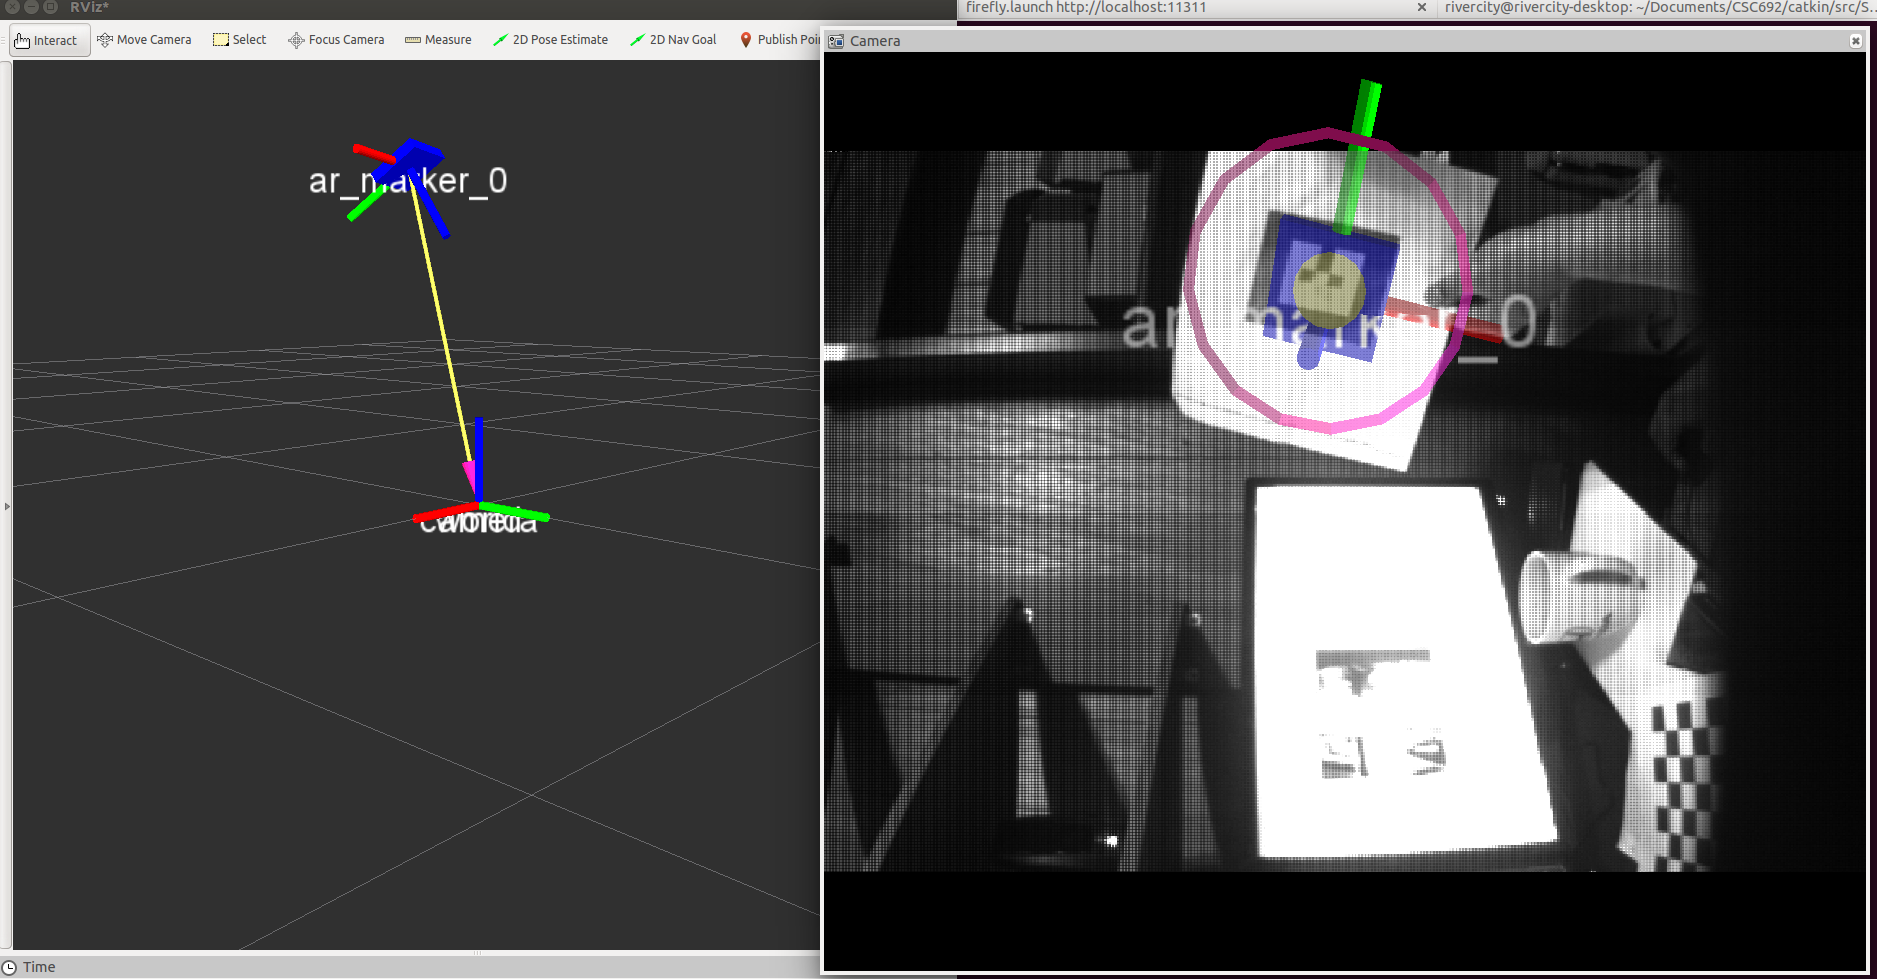
\includegraphics[width=.75\textwidth]{images/tracker}
\label{tracker}
\end{figure} 

Before leaving discussion of this package, we will review the graph of topic communication seen in figure ~\ref{tracker_graph}. We see that ar\_track\_alvar subscribe to both image\_raw and camera\_info topics. The node then passes that information to tf to calculate the pose of the tag relative to the camera frame. In the launch file you may have noticed the tf call.
\begin{lstlisting}[language=xml]
	<node pkg="tf" type="static_transform_publisher" name="map_to_camera" output="screen" args="0 0 0 0 0 0 world camera 10" />
\end{lstlisting}
This is providing us the ability to set the transform, as well as adjust the alignment of the pose in the argument list. These arguments are, in order:
\begin{itemize}
\item x offset in meters
\item y offset in meters
\item z offset in meters
\item yaw in radians
\item pitch in radians
\item roll in radians
\item frame\_id
\item child\_frame\_id
\item frequency of sending the tf message in milliseconds
\end{itemize}
Also present, but not appearing on the graph, are the published topics for the tag pose and the marker visualization. These topics will remain 'silent' until there is another node subscribes to those topics. 
\begin{figure}[h]
\caption{Graph of communications with ar\_track\_alvar}
\centering
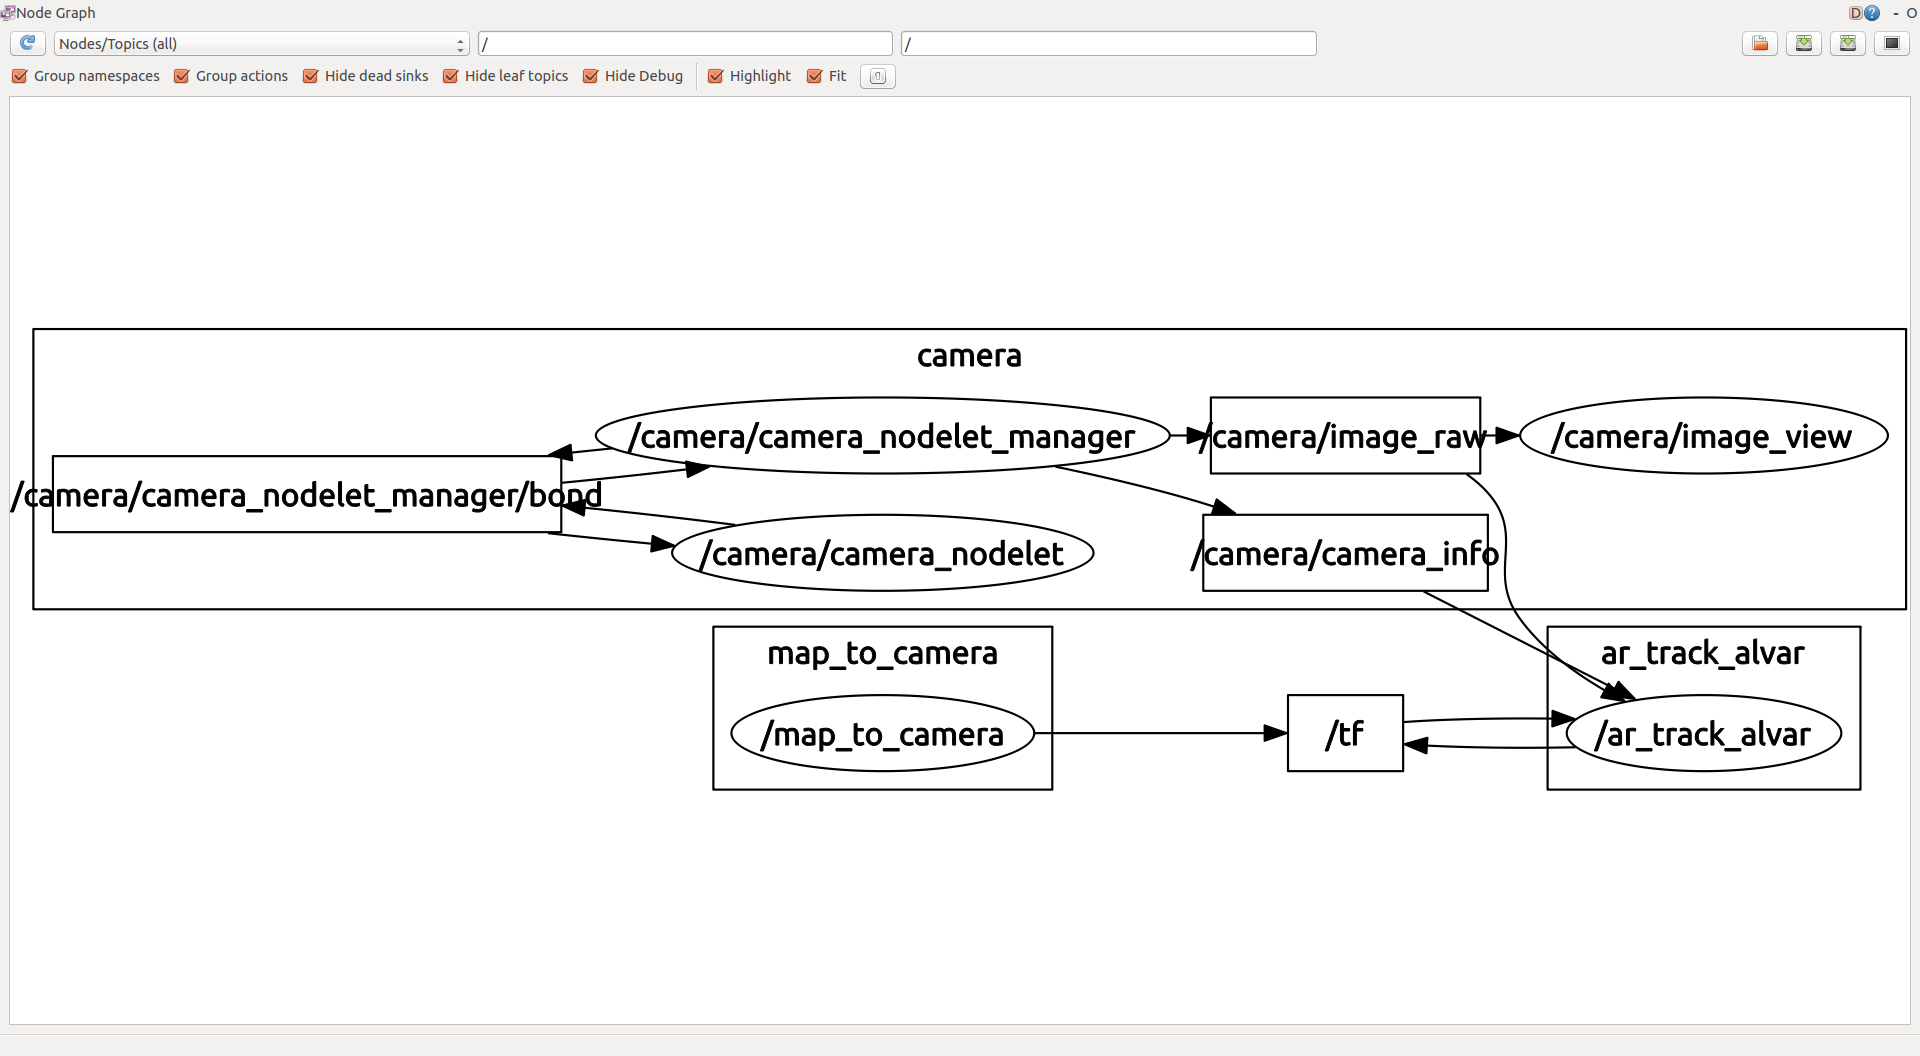
\includegraphics[width=.75\textwidth]{images/tracker_graph}
\label{tracker_graph}
\end{figure} 
\end{itemize}

\subsection{Localization}
\noindent \textbf{svo}:Localization is the backbone of pose estimation. The downside to relying upon a GPS localization is that in an area with weak or no GPS signal (indoors, near buildings, in canyons or ravines), the pose estimate becomes poor or useless. Without reliable pose information, the UAV is unable to solely rely upon its IMU data to judge its movements.\\

\begin{itemize}
\item License: GPLv3
\item Documentation: \url{https://github.com/uzh-rpg/rpg_svo/wiki}
\item Source: \url{https://github.com/uzh-rpg/rpg_svo}
\item Parameters
\begin{itemize}
\item trace\_name: Base-name of the tracefiles. \\
\textit{param data type}: string

\item trace\_dir: Directory where the tracefiles are saved.	 \\
\textit{param data type}: string

\item n\_pyr\_levels: Number of pyramid levels used for features.	 \\
\textit{param data type}: integer

\item use\_imu: Use the IMU to get relative rotations. \\
\textit{param data type}: boolean

\item core\_n\_kfs:	Number of keyframes in the core. The core-kfs are optimized through bundle adjustment. \\
\textit{param data type}: integer

\item map\_scale: Initial scale of the map. Depends on the distance the camera is moved for the initialization.	 \\
\textit{param data type}: double

\item grid\_size: Feature grid size of a cell in [px].	 \\
\textit{param data type}: integer

\item init\_min\_disparity: Initialization: Minimum required disparity between the first two frames.	 \\
\textit{param data type}: double

\item init\_min\_tracked: Minimum number of tracked features.	 \\
\textit{param data type}: integer

\item init\_min\_inliers: Minimum number of inliers after RANSAC.	 \\
\textit{param data type}: integer

\item klt\_max\_level: Maximum level of the Lucas Kanade tracker.	 \\
\textit{param data type}: integer

\item klt\_min\_level: Minimum level of the Lucas Kanade tracker.	 \\
\textit{param data type}: integer

\item reproj\_thresh: Reprojection threshold [px].	 \\
\textit{param data type}: double

\item poseoptim\_thresh:	Reprojection threshold after pose optimization. \\
\textit{param data type}: double

\item poseoptim\_num\_iter:	Number of iterations in local bundle adjustment. \\
\textit{param data type}: integer

\item structureoptim\_max\_pts: Maximum number of points to optimize at every iteration.	 \\
\textit{param data type}: integer

\item structureoptim\_num\_iter:	Number of iterations in structure optimization. \\
\textit{param data type}: integer

\item loba\_thresh: Reprojection threshold after bundle adjustment.	 \\
\textit{param data type}: double

\item loba\_robust\_huber\_width: Threshold for the robust Huber kernel of the local bundle adjustment.	 \\
\textit{param data type}: double

\item loba\_num\_iter: Number of iterations in the local bundle adjustment.	 \\
\textit{param data type}: integer

\item kfselect\_mindist:	Minimum distance between two keyframes. Relative to the average height in the map. \\
\textit{param data type}: double

\item triang\_min\_corner\_score: Select only features with a minimum Harris corner score for triangulation.	 \\
\textit{param data type}: double

\item triang\_half\_patch\_size:	Subpixel refinement of reprojection and triangulation. Set to 0 if no subpix refinement required! \\
\textit{param data type}: integer

\item  max\_n\_kfs:	Limit the number of keyframes in the map. This makes nslam essentially a Visual Odometry. Set to 0 if unlimited number of keyframes are allowed. Minimum number of keyframes is 3. \\
\textit{param data type}: integer

\item img\_imu\_delay: How much (in milliseconds) is the camera delayed with respect to the imu. \\
\textit{param data type}: double

\item max\_fts: Maximum number of features that should be tracked.	 \\
\textit{param data type}: integer

\item quality\_min\_fts:	 If the number of tracked features drops below this threshold. Tracking quality is bad. \\
\textit{param data type}: integer

\item quality\_max\_drop\_fts: If within one frame, this amount of features are dropped. Tracking quality is bad. \\
\textit{param data type}: integer
\end{itemize}

\item Subscribed Topics
\begin{itemize}
\item <camera\_topic\_node>/image\_raw: image frames from camera
\end{itemize}
\item Published Topics
\begin{itemize}
\item /svo/dense\_input
\item /svo/image
\item /svo/info
\item /svo/keyframes
\item /svo/points
\item /svo/pose: this is the pose estimate with x,y,z coordinates, along with orientation as a quaternion. 
\item /svo/remote\_key

\end{itemize}

\item Installation:\\

Installation of this package is a bit different from the previous package installation instructions, and a bit more involved.\\

\textbf{Step by Step}:
\begin{enumerate}
\item create a workspace for two CMake projects
\begin{lstlisting}[language=bash]
$ mkdir vis_workspace
\end{lstlisting}
\item install our first project, Sophus
\begin{lstlisting}[language=bash]
$ cd vis_workspace
$ git clone https://github.com/strasdat/Sophus.git
$ cd Sophus
$ git checkout a621ff
$ mkdir build
$ cd build
$ cmake ..
$ make
\end{lstlisting}
Sophus (by Hauke Strasdat) implements Lie groups which are needed to describe rigid body transforms. \\ 

\item install the second project, Fast
\begin{lstlisting}[language=bash]
$ cd vis_workspace
$ git clone https://github.com/strasdat/Sophus.git
$ cd Sophus
$ git checkout a621ff
$ mkdir build
$ cd build
$ cmake ..
$ make
\end{lstlisting}
This is the Fast corner detector by Edward Rosten, which is needed to quickly find features in the image.\\

\item make a catkin workspace if one is not available
\begin{lstlisting}[language=bash]
$ mkdir vis_catkin
$ cd vis_catkin
$ mkdir src
$ src
$ catkin_init_workspace
\end{lstlisting}
\item let's install vikit
\begin{lstlisting}[language=bash]
$ cd vis_catkin/src
$ git clone https://github.com/uzh-rpg/rpg_vikit.git
\end{lstlisting}
vikit contains lots of tools which are required for SVO such as camera models and interpolation functions.\\

\item now for SVO!
\begin{lstlisting}[language=bash]
$ cd vis_catkin/src
$ git clone https://github.com/uzh-rpg/rpg_svo.git
\end{lstlisting}
\item before we go any further, let's make sure we have our cmake modules
\begin{lstlisting}[language=bash]
$ sudo apt-get install ros-jade-cmake-modules
\end{lstlisting}
\item now let's build
\begin{lstlisting}[language=bash]
$ cd vis_catkin
$ catkin_make
\end{lstlisting}
\item Before running the launch file
\begin{enumerate}
\item have the correct camera calibration file located in the folder located at\\ <catkin\_space>/src/rpg\_svo/param
\item have the vo\_px4.yaml file created in that same folder location as the camera calibration file. This is most easily achieved by making a copy of the vo\_fast.yaml file located there and renaming it.
\end{enumerate}
\end{enumerate}

\item Launch File \& Usage:\\

Before launching SVO, be sure to start the camera, so that the appropriate topics are published and advertised, so that SVO will be able to subscribe to the image topic.\\ 
\begin{lstlisting}[language=xml]
<launch>
  
    <node pkg="svo_ros" type="vo" name="svo" clear_params="true" output="screen">
    
        <!-- Camera topic to subscribe to -->
        <param name="cam_topic" value="/camera/image_raw" type="str" />
        <param name="max_fts" value="200" type="int" />
        <param name="min_fts" value="20" type="int" />
        <param name="init_min_disparity" value="10.0" type="double" />
        
        <!-- Camera calibration file -->
        <rosparam file="$(find svo_ros)/param/firefly.yaml" />
        
        <!-- Default parameter settings: choose between vo_fast and vo_accurate -->
        <rosparam file="$(find svo_ros)/param/vo_px4.yaml" />

    </node>
        
</launch>	
\end{lstlisting}
To use this launch file, there are at least two files that must be modified or created to use this package.\\
\begin{itemize}
\item The first file that will need to be created is the <camera>.yaml file. For our implementation, this is the firefly.yaml file. To make this file, we can use the calibration file that was created earlier (the firefly calibration is used here). 
\begin{lstlisting}[language=xml]
image_width: 640
image_height: 480
camera_name: 0
camera_matrix:
  rows: 3
  cols: 3
  data: [502.0479811571255, 0, 328.3379912823597, 0, 502.5040566931246, 249.276443286676, 0, 0, 1]
distortion_model: plumb_bob
distortion_coefficients:
  rows: 1
  cols: 5
  data: [-0.3385831965124953, 0.1221738505255268, -0.000681702092234282, 0.0005802657058398539, 0]
rectification_matrix:
  rows: 3
  cols: 3
  data: [1, 0, 0, 0, 1, 0, 0, 0, 1]
projection_matrix:
  rows: 3
  cols: 4
  data: [424.6744384765625, 0, 331.5108446465238, 0, 0, 459.6941223144531, 250.1992172933205, 0, 0, 0, 1, 0]
\end{lstlisting}
We first need the image height and width, which should be fairly obvious. Next we need the camera model where the camera\_matrix statistics in the above example is more easily discernible as:
\\
\vspace{2mm}\\
$
\begin{bmatrix}
    cam\_fx  &  	0 	 & cam\_cx \\
    0	    & cam\_fy & cam\_cy \\
    0	    & 0 & 1
\end{bmatrix}
$\\
\vspace{2mm}\\
Next, the distortion\_cofficients data array will compose the cam\_d0 to cam\_d4. With these values we can create a calibration file that meets the format requirements of svo.\\
We just need to create a file named <camera>.yaml and fill it with the following information:
\begin{lstlisting}[language=python]
cam_model: Pinhole
cam_width: 640
cam_height: 480
cam_fx: 502.047981
cam_fy: 502.504057
cam_cx: 328.337991
cam_cy: 249.276443
cam_d0: -0.338583
cam_d1: 0.122174
cam_d2: -0.000682
cam_d3: 0.000580
\end{lstlisting}
We make this a Pinhole camera, as the pinhole camera type is the most similar to the model of the camera we are using. The supported types are:
\begin{itemize}
\item ATAN - Uses FOV distortion model, and is the preferred model by the authors of this package. The authors state that this model computes projections much faster than other camera models. Requires the ethzasl\_ptam calibration tool.
\item Pinhole - Standard model for OpenCV and ROS. Requires the camera\_calibration tool to determine calibration parameters.
\item Ocam - Used to model cameras with high field of view and omnidirectional cameras. Requires the OCamCalib to determine calibration parameters.
\end{itemize} 
\item The second file that is required is the vo\_px4.yaml.
\begin{lstlisting}[language=python]
grid_size: 30
max_n_kfs: 20
loba_num_iter: 5
max_fts: 180
\end{lstlisting}
This file contains parameter information that is read and set at instantiation of the svo node. This example is the file we are using and does the following: 
\begin{itemize}
\item sets the grid size of a single cell to be 30 pixels square.
\item sets the maximum number of keyframes to 20.
\item caps the number of iterations in the bundle adjustment to 5.
\item caps the number of features tracked to 180.
\end{itemize}
\end{itemize}
In running this program, the SVO package will gather up a number of features and initialize this point as the origin for its pose. Outputting the pose information will look much like the pose displayed on the terminal in figure ~\ref{svo}. This example is taken immediately after localization is achieved, and so our coordinates are very close to the origin.\\

\begin{figure}[H]
\caption{SVO pose example}
\centering
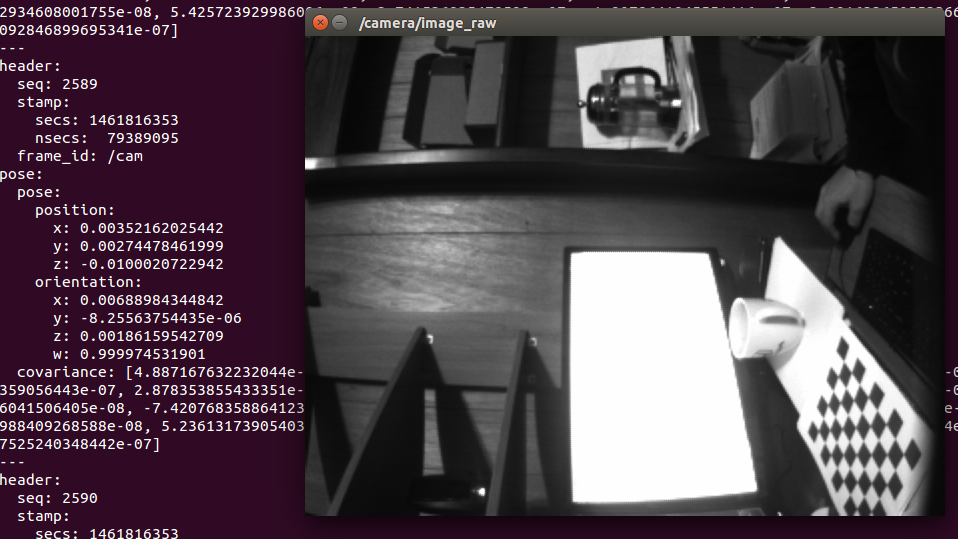
\includegraphics[width=.75\textwidth]{images/svo}
\label{svo}
\end{figure} 

Looking at our communication graph in figure ~\ref{svo_graph}, we see the camera namespace. This namespace is publishing the image topics, which are being subscribed to by both ar\_track\_alvar and svo nodes. Both nodes send this to the tf node to estimate the pose of the UAV and the pose of the AR tag. \\

\begin{figure}[h]
\caption{Graph of communications with SVO}
\centering
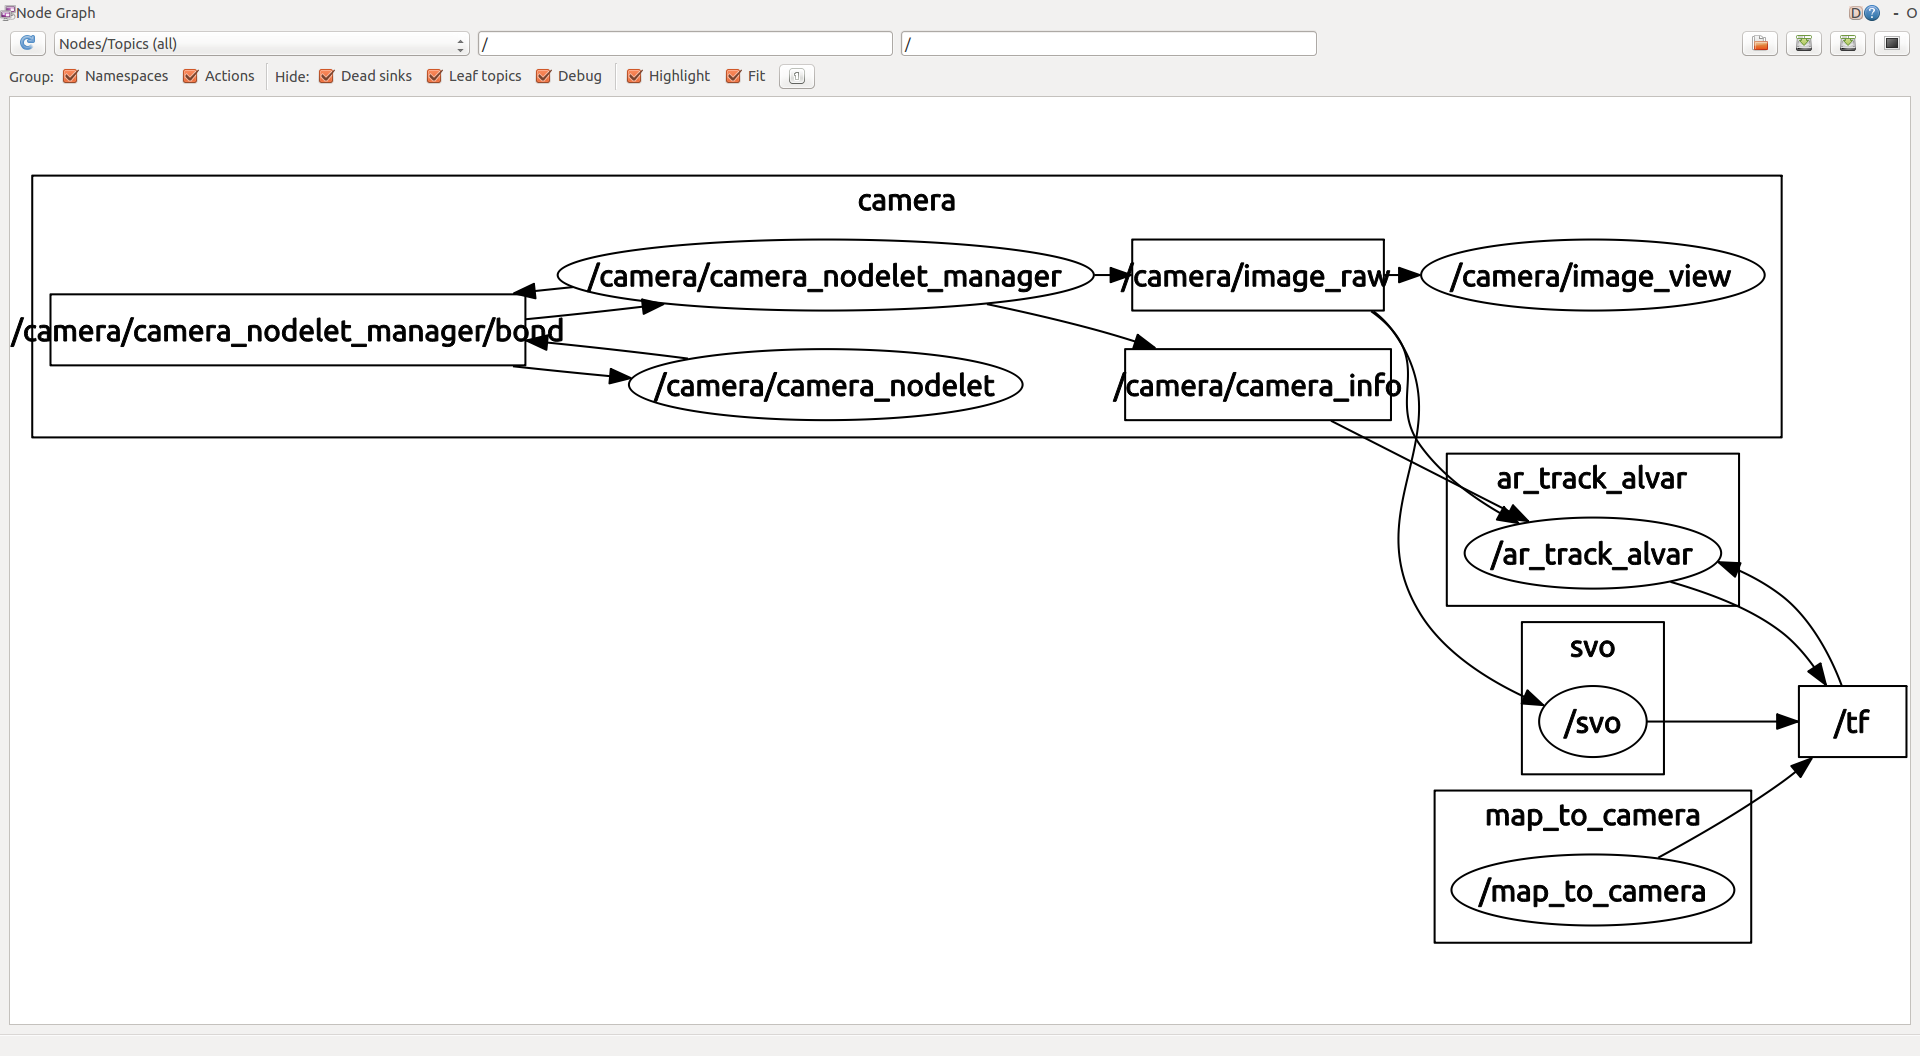
\includegraphics[width=.75\textwidth]{images/svo_graph}
\label{svo_graph}
\end{figure} 

Unfortunately, we found that SVO is extremely fragile in our implementation. Robust performance and reliable results are not guaranteed by the authors of the package, and we found that the camera could only be moved slightly before losing localization due to a loss of tracked features. This is demonstrated in figure ~\ref{svo_break}.\\
 
\begin{figure}[H]
\caption{SVO failing to localize}
\centering
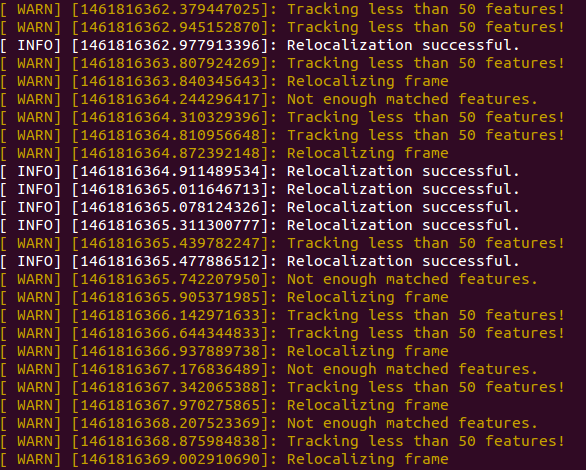
\includegraphics[width=.5\textwidth]{images/svo_break}
\label{svo_break}
\end{figure} 

The team feels that the promise of localization is worth the investment with this package. Likely culprits may be slow processing of pose relative to the number of frames being sent. Another issue may be the camera is not achieving crisp (clear, not blurry, images), which would make feature matching that much more difficult. The answer may lay in playing with the various parameters respective of current image processing ability.
\end{itemize}
